% Matteo Kumar - Leonard Schatt
% Physikalisches Praktikum

% Anhang A

\chapter{Anhang}
\label{chap:anhangA}
\section{Methodik}
\subsection{Versuchsaufbauten}
\subsubsection{Aufbau spektrale Empfindlichkeit}

\begin{figure}[h]
    \centering
    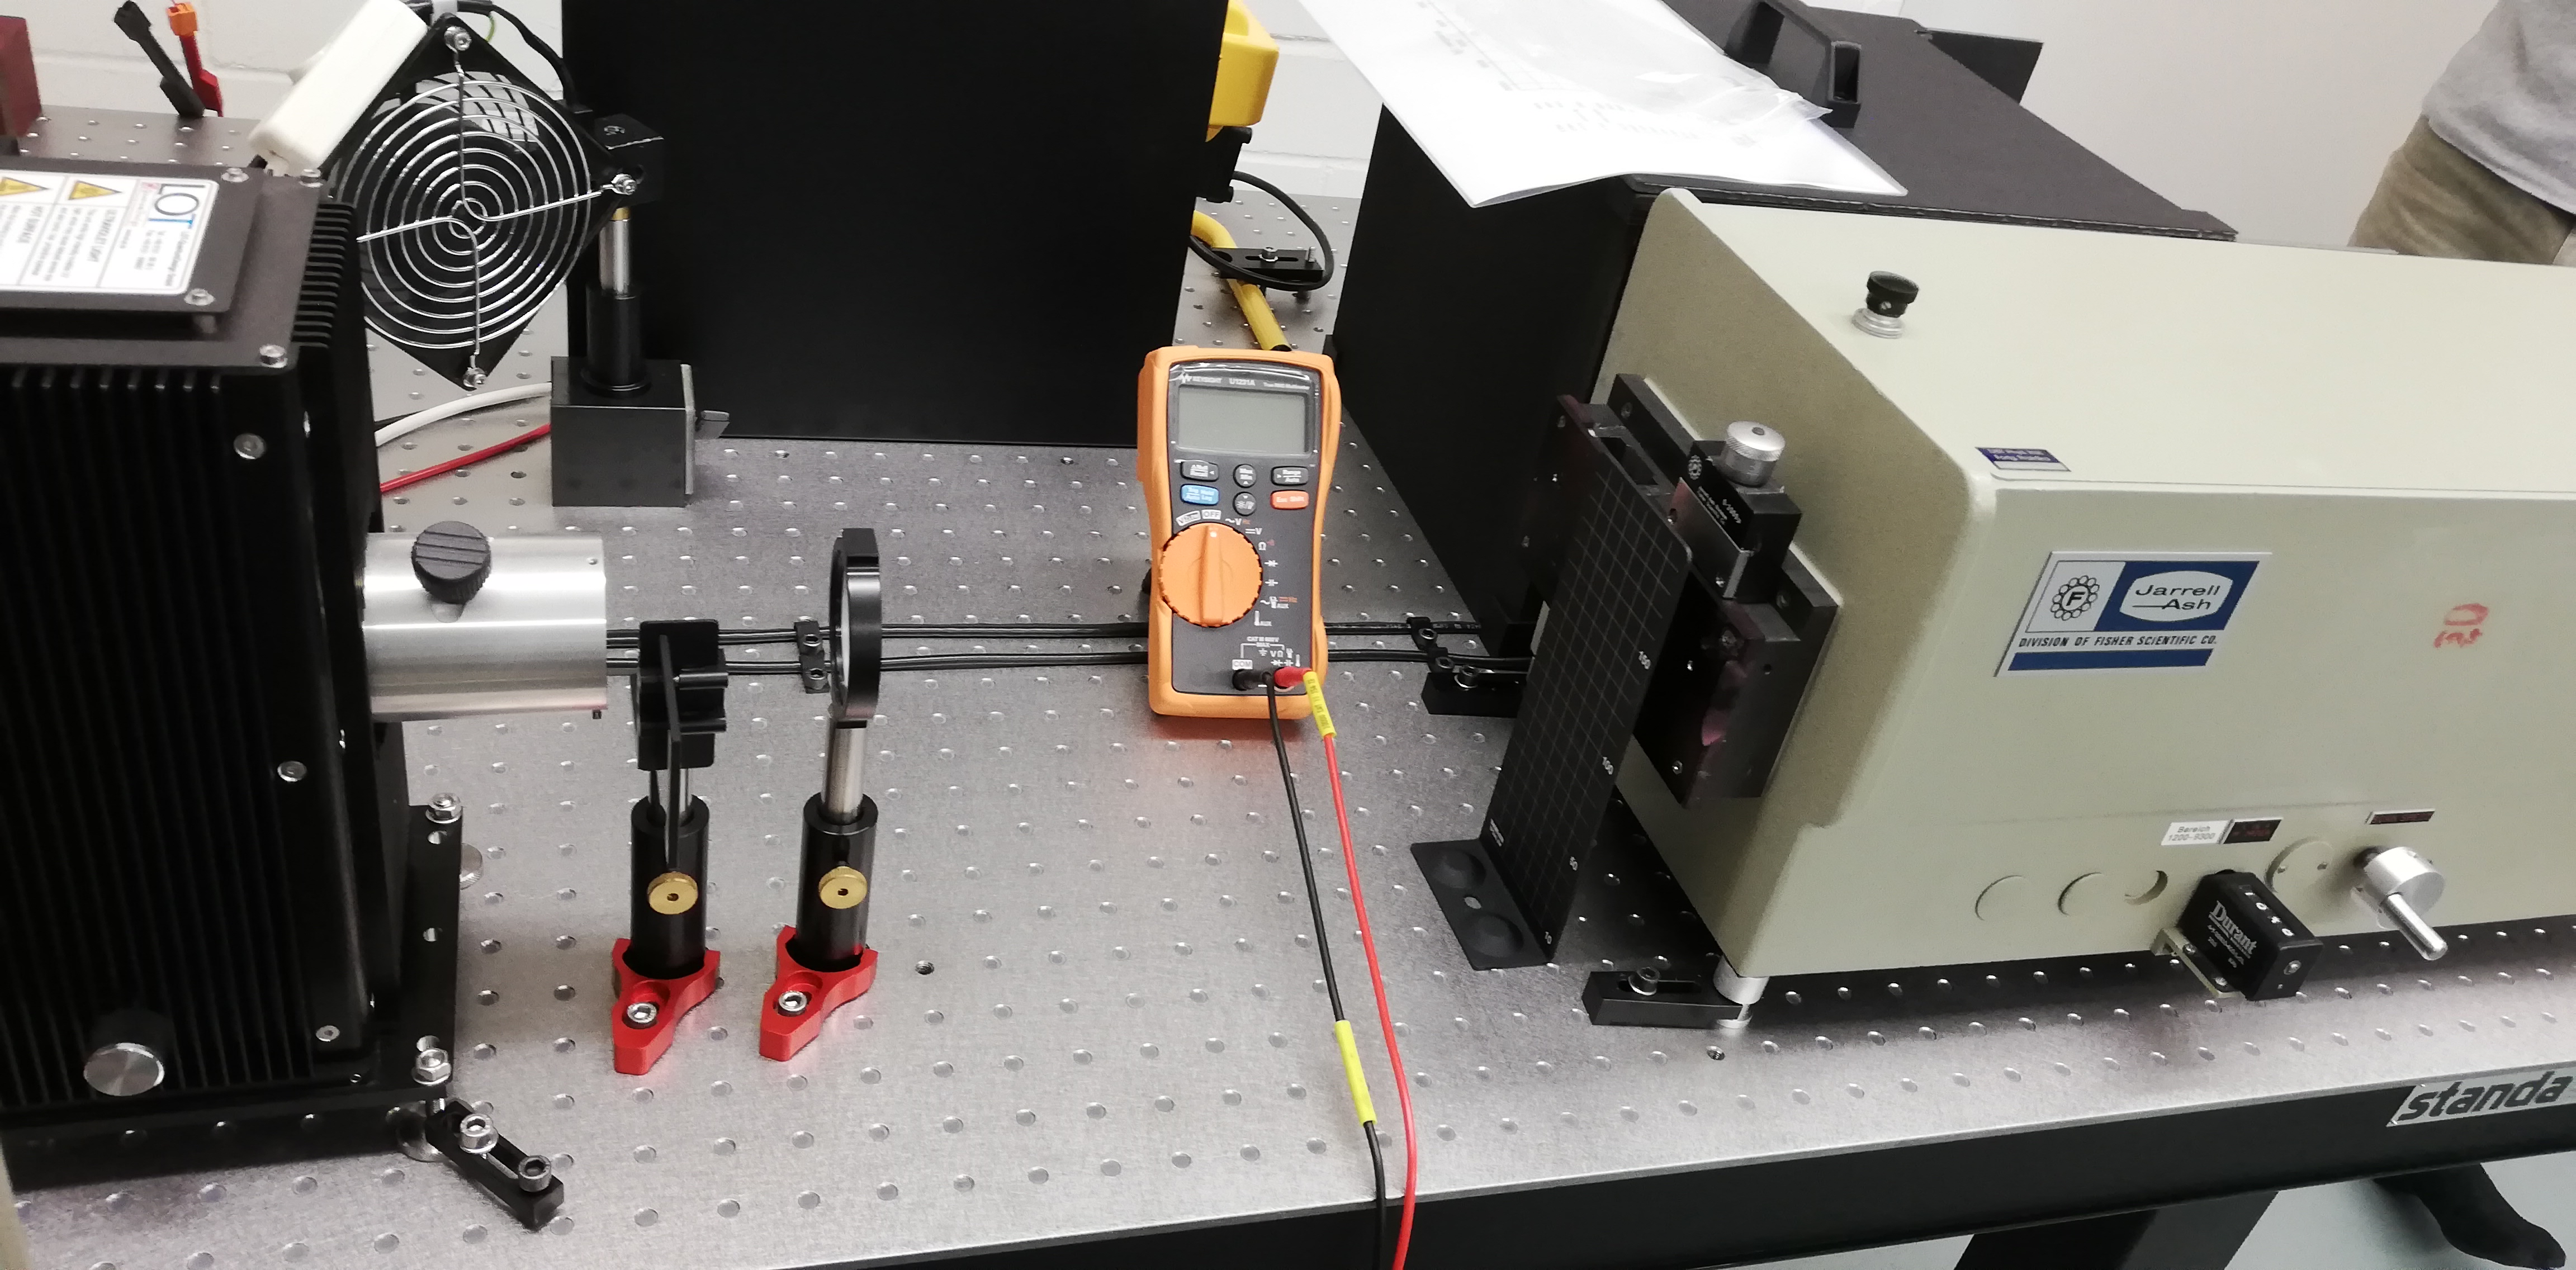
\includegraphics[width = \linewidth]{Bilder/Aufbau6.jpg}
    \caption{Xenon-Lampe mit vorgelagertem Filter}
\end{figure}

\begin{figure}[h]
    \centering
    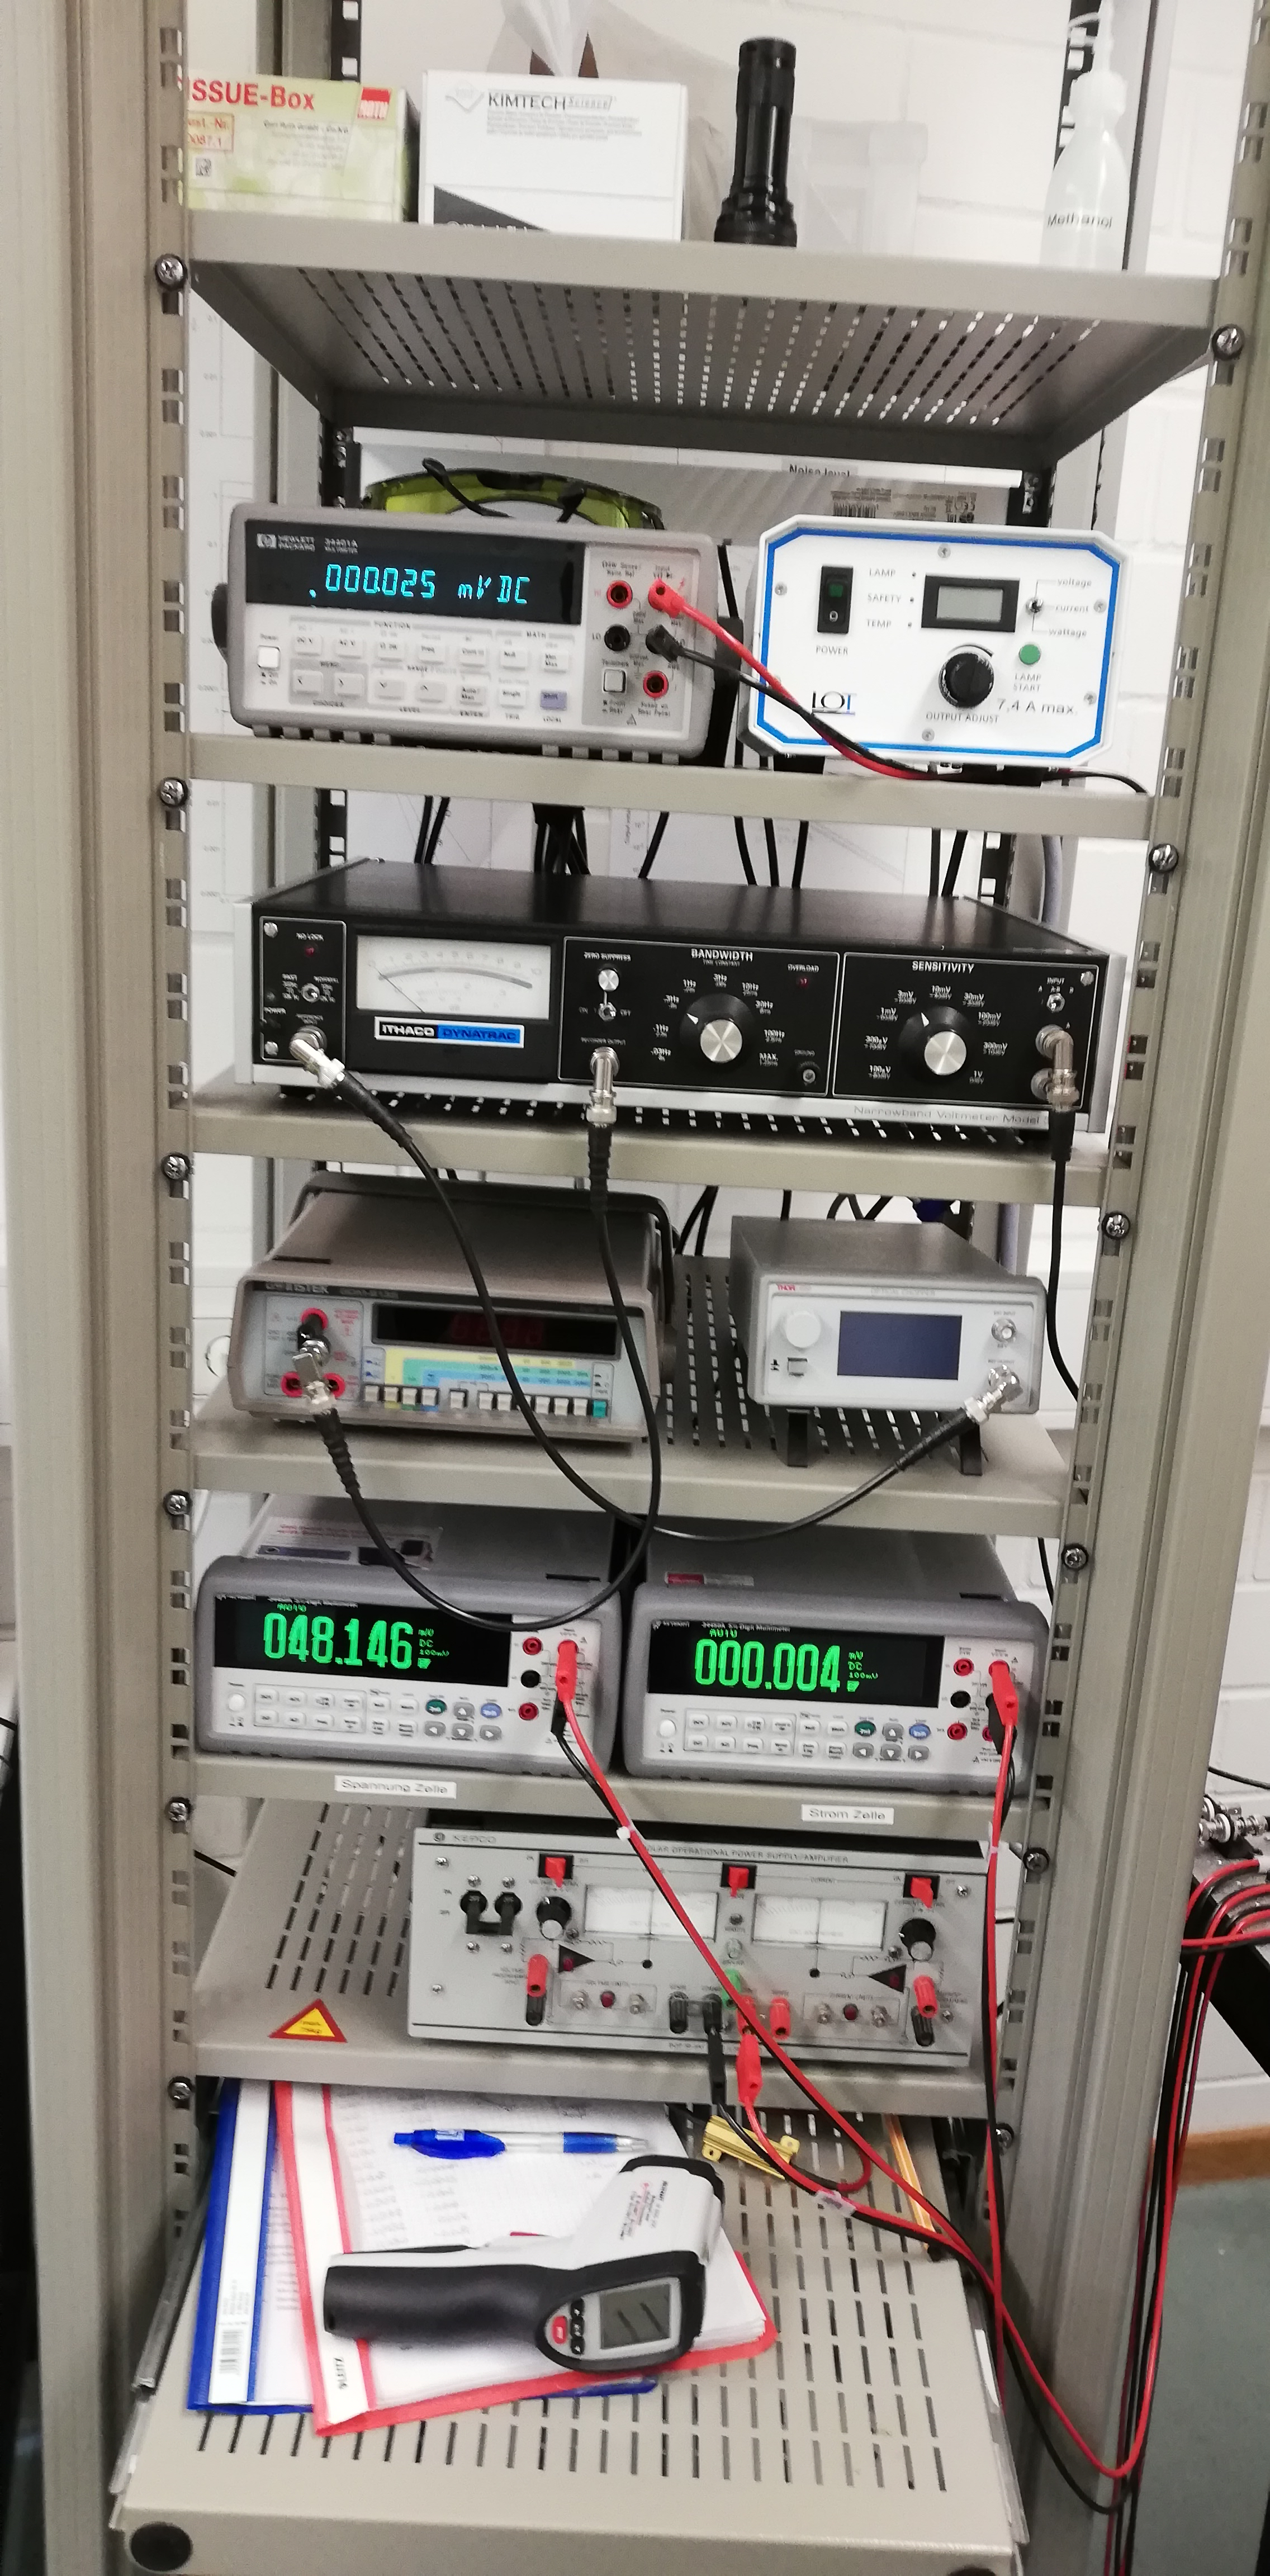
\includegraphics[width = 8cm]{Bilder/Aufbau3.jpg}
    \caption{Verwendete Messgeräte (in schwarz der Lock-in Verstärker)}
\end{figure}

\begin{figure}[h]
    \centering
    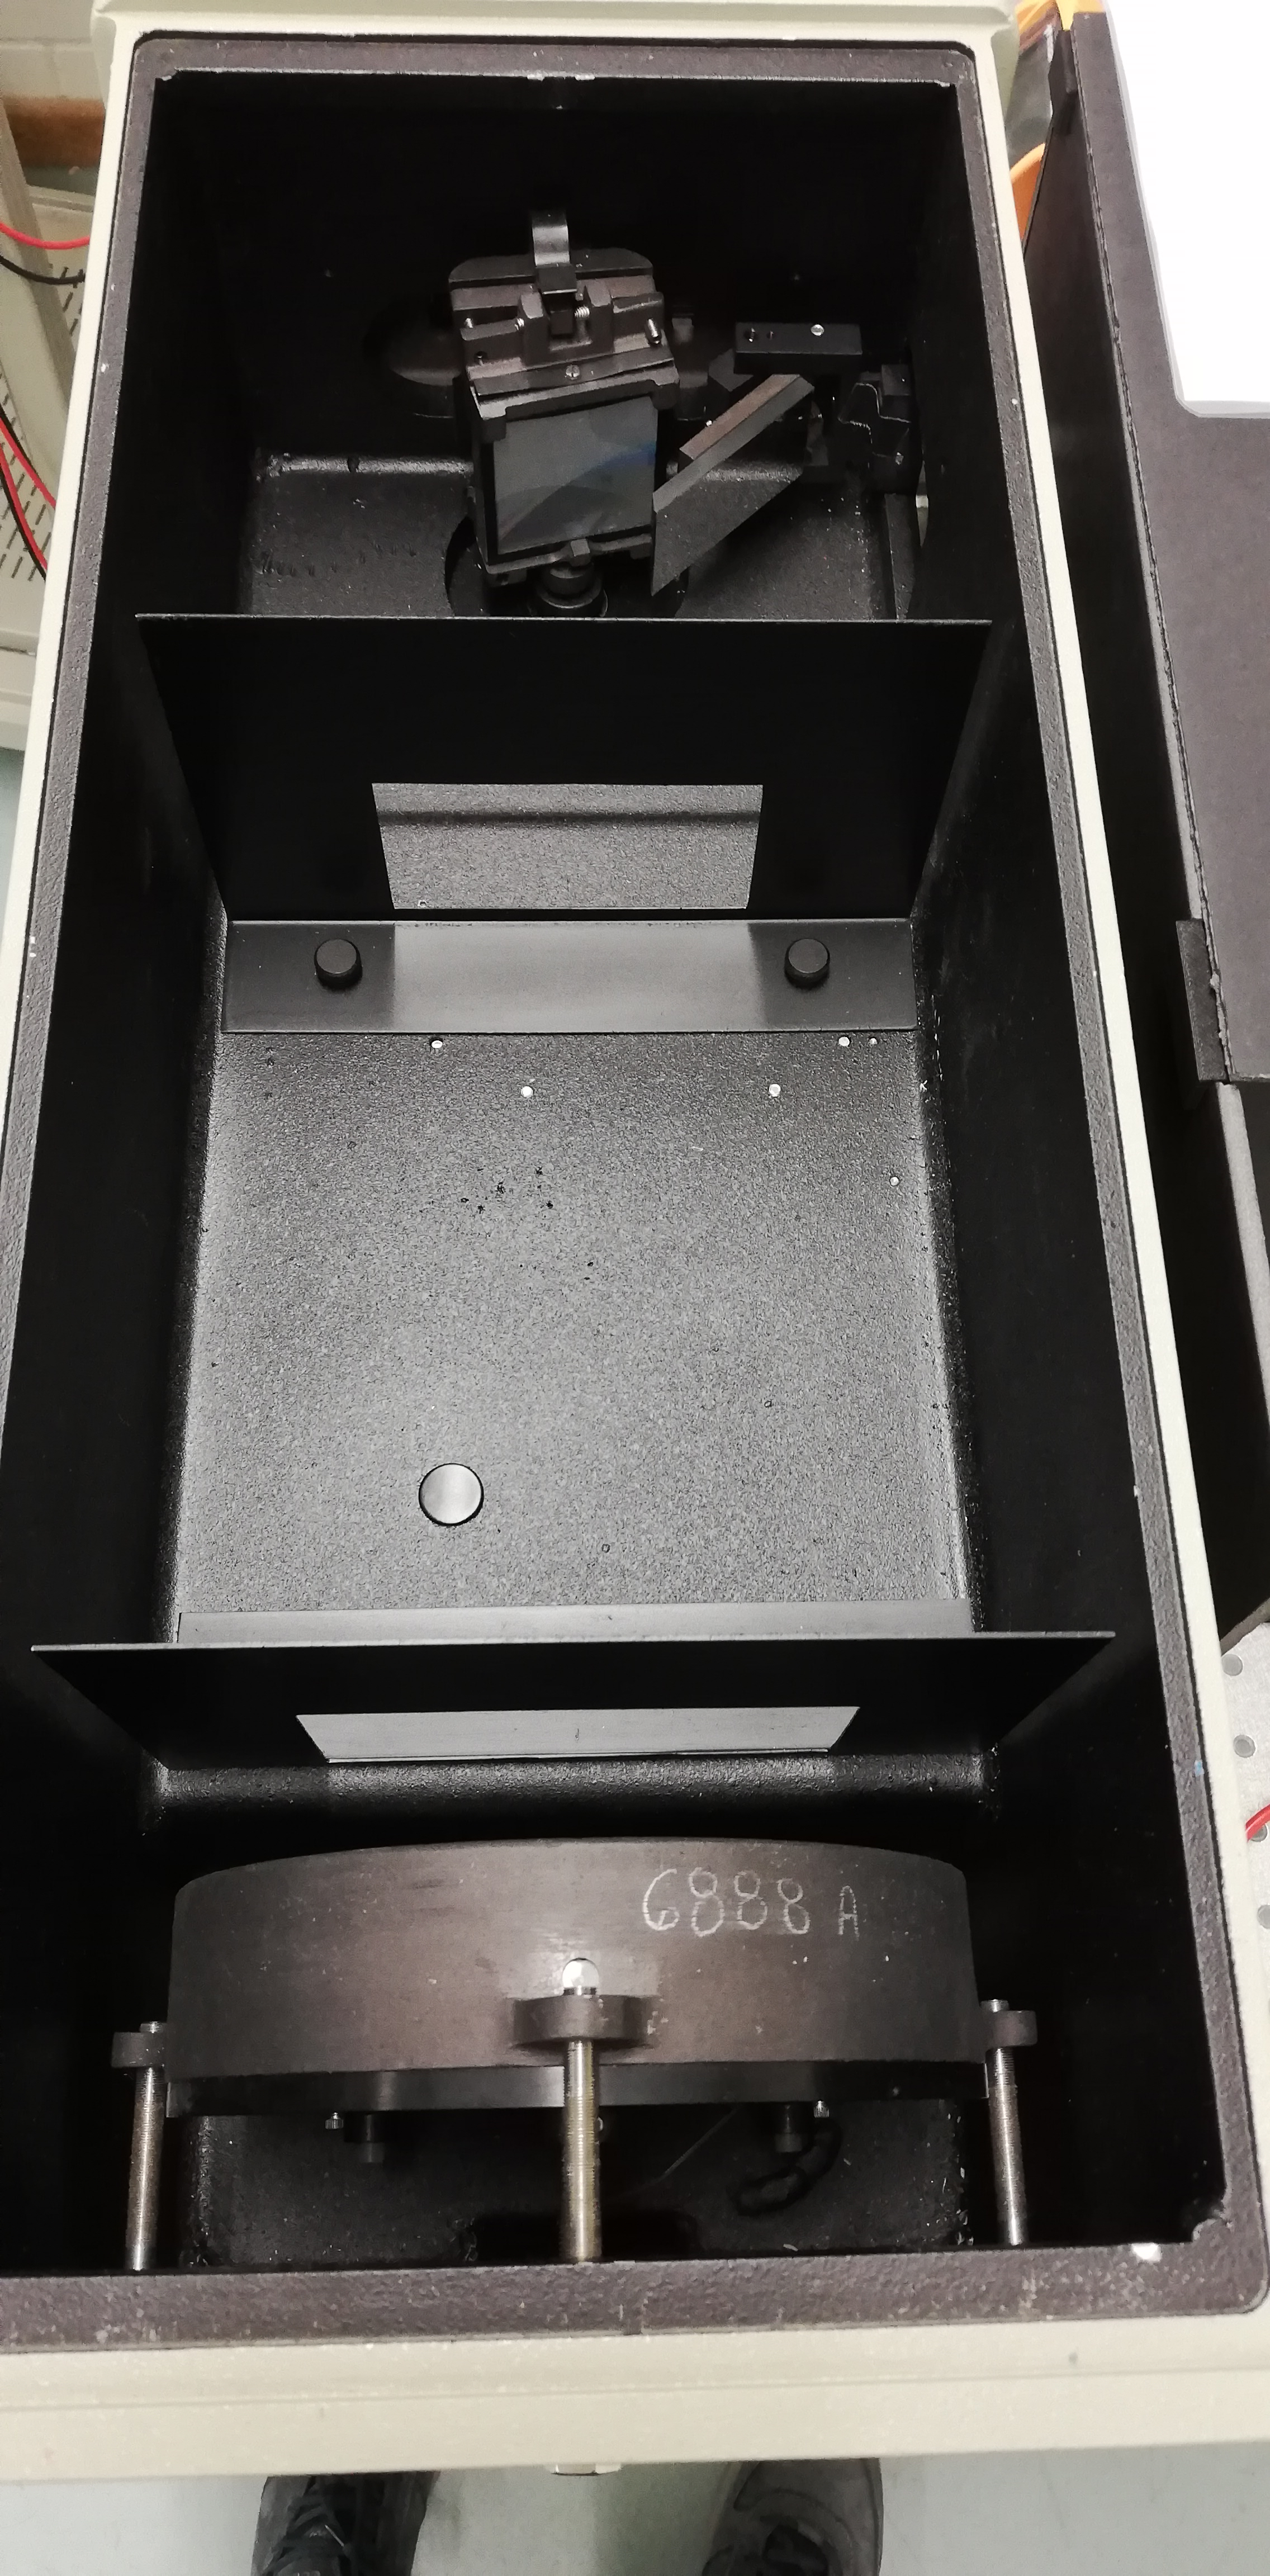
\includegraphics[width = 8cm]{Bilder/Aufbau4.jpg}
    \caption{Innenansicht des Gitterspektrometers}
\end{figure}
\clearpage


\subsubsection{Versuchsteil U-I-Kennlinien}

\begin{figure}[h]
    \centering
    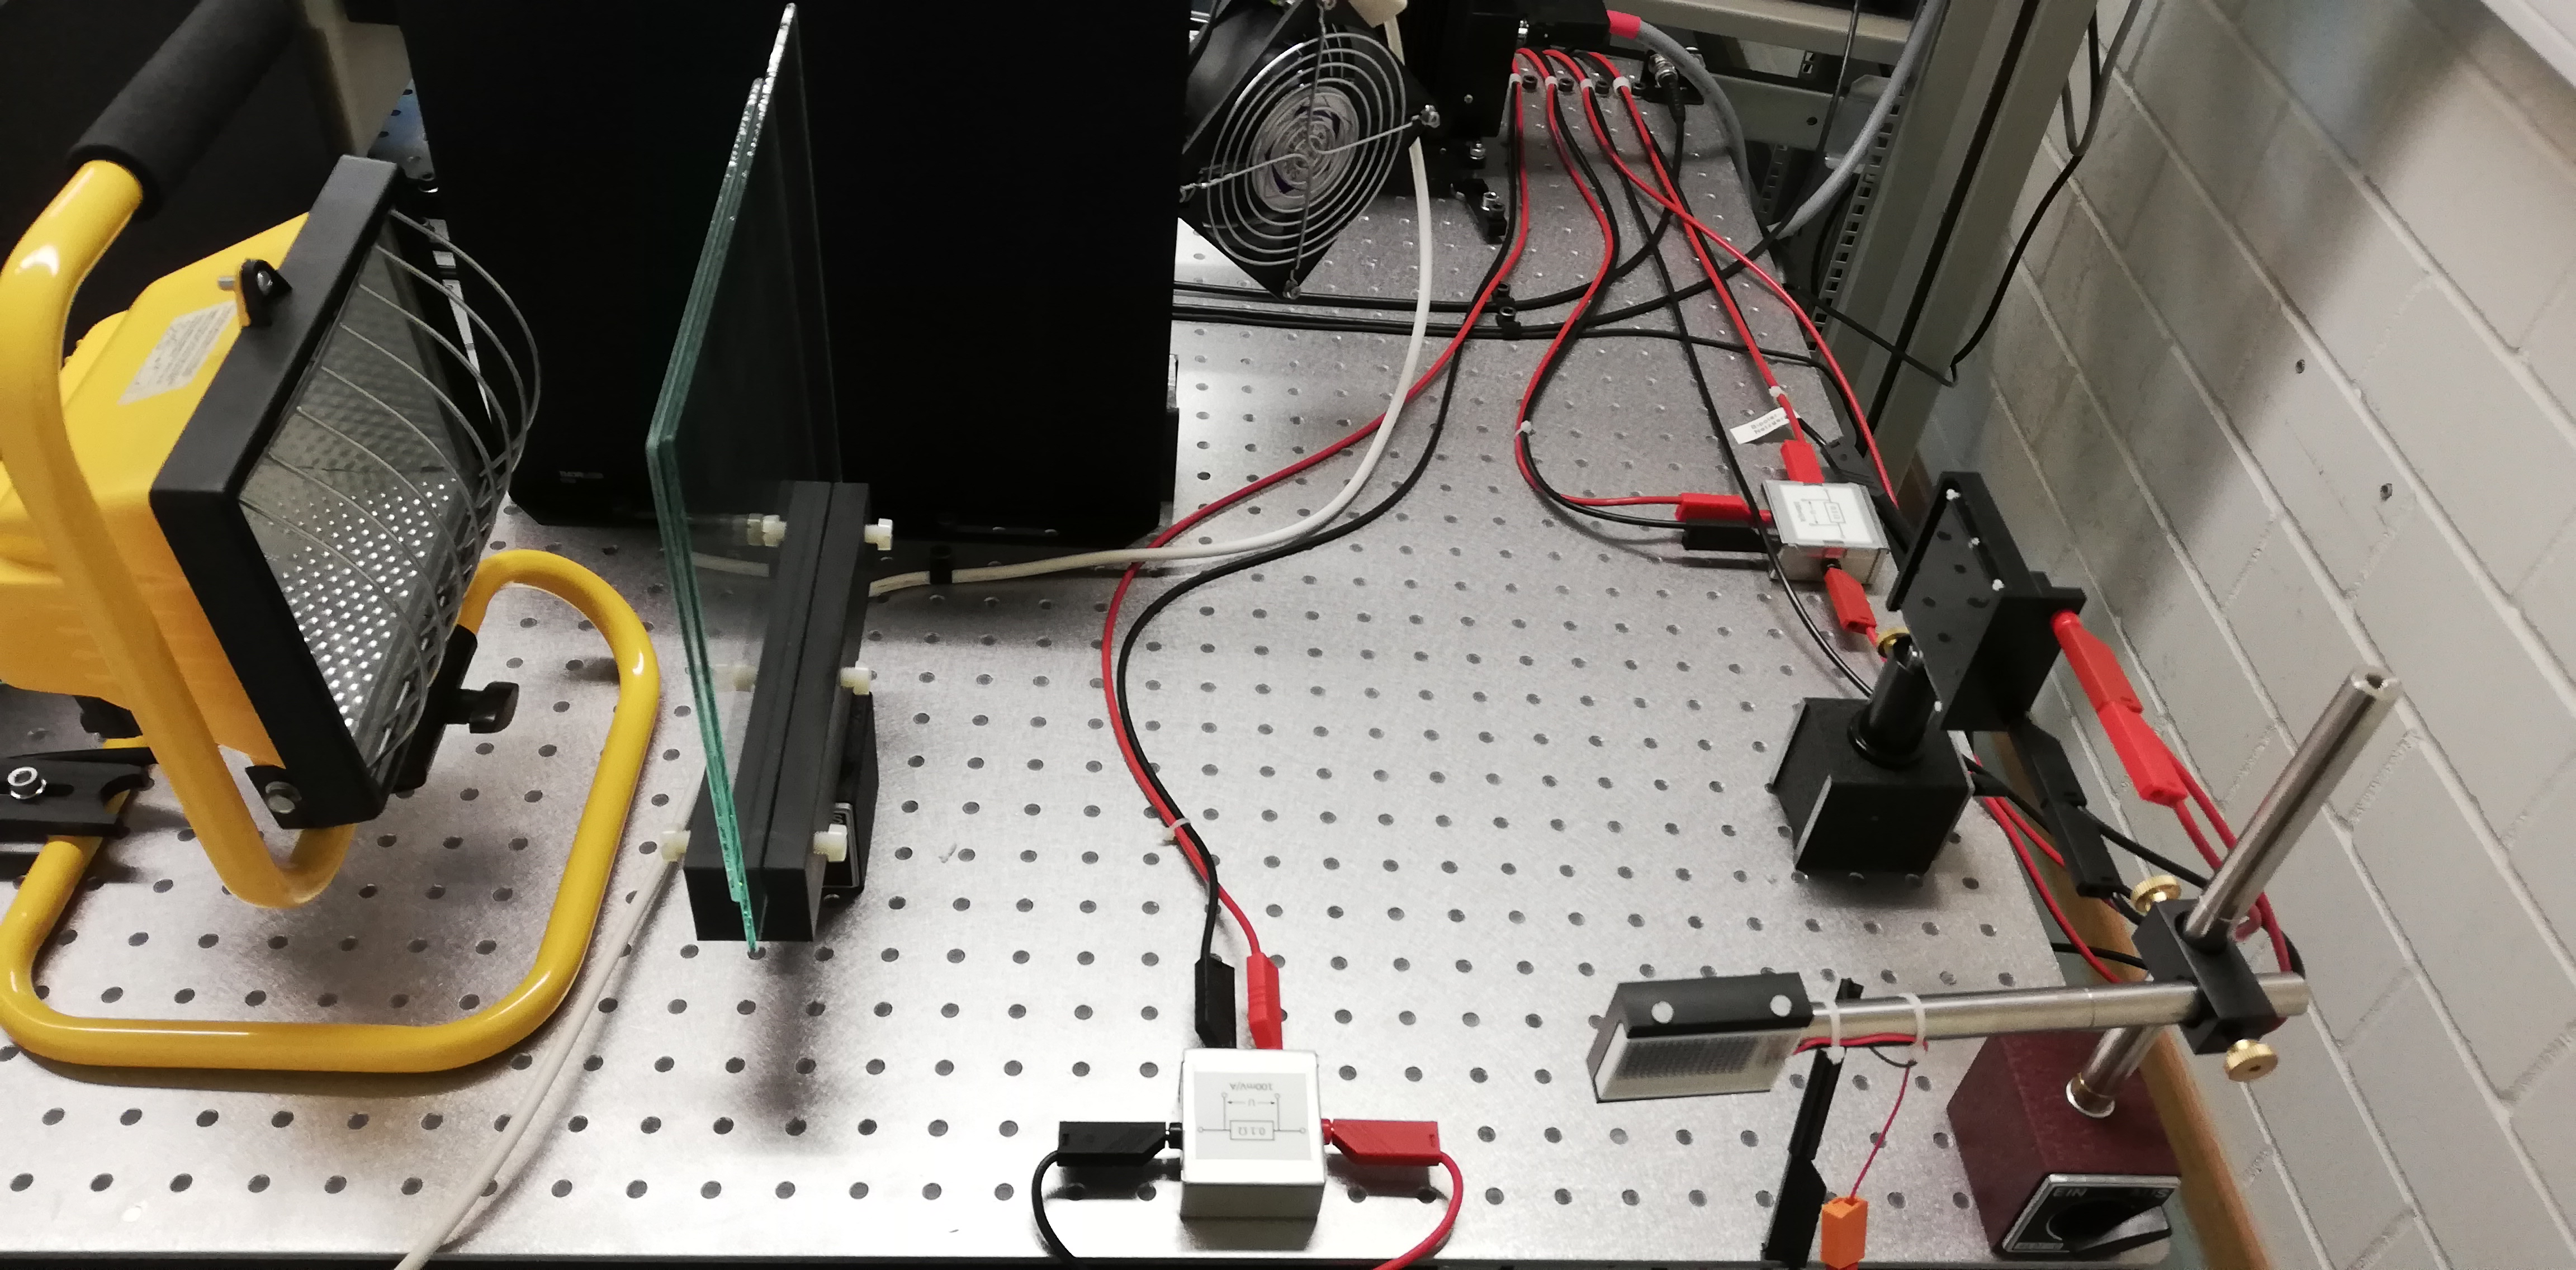
\includegraphics[width = \linewidth]{Bilder/Aufbau1.jpg}
    \caption{Baustrahler mit vorgelagerten Glasplatten}
\end{figure}


\clearpage

\section{Fitten der Shockley-Gleichung}
\label{section:AnhangShock}

\begin{figure}[ht]
    \centering
    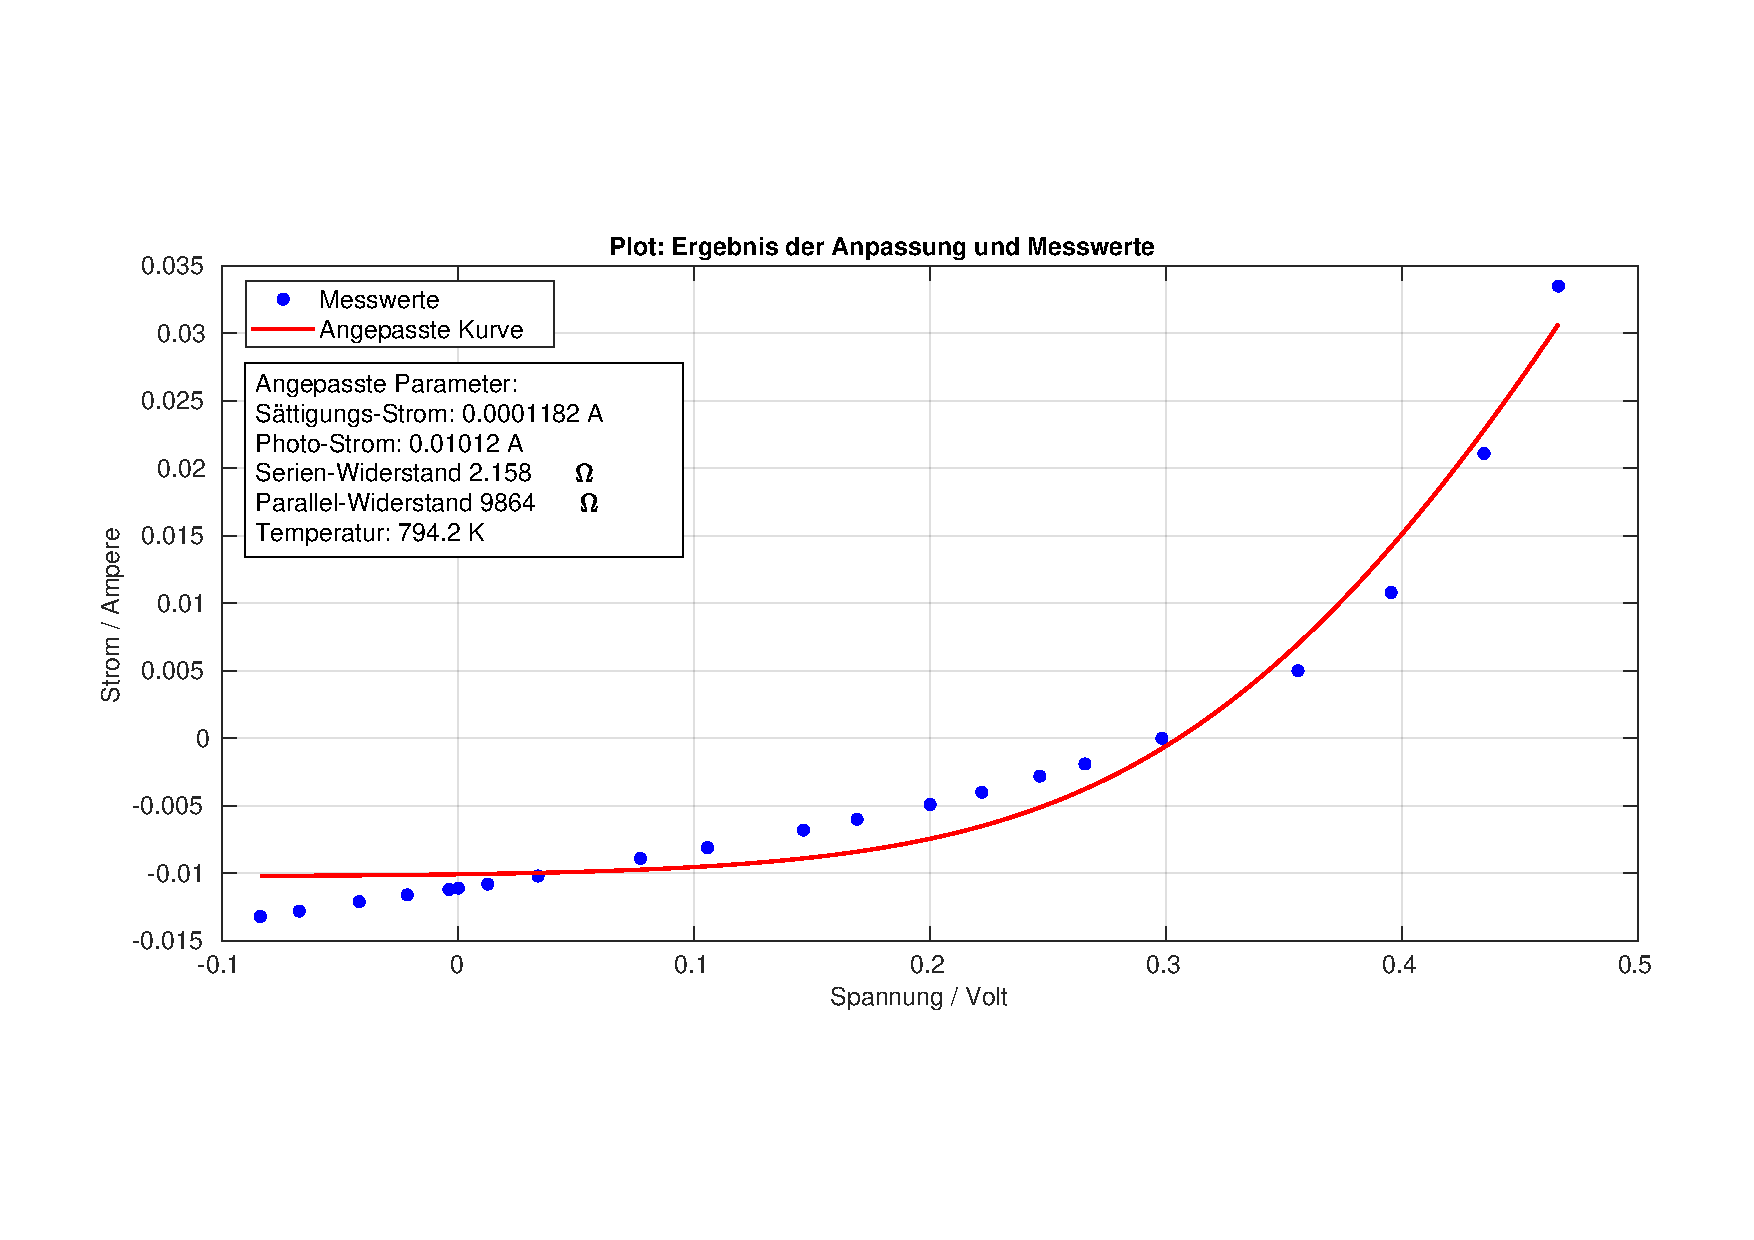
\includegraphics[width = \linewidth]{Bilder/CIS180Plot.pdf}
    \caption{Gefittete Shockley-Gleichung an das CIS-Modul bei 180V Trafospannung}    
\end{figure}

\begin{figure}[ht]
    \centering
    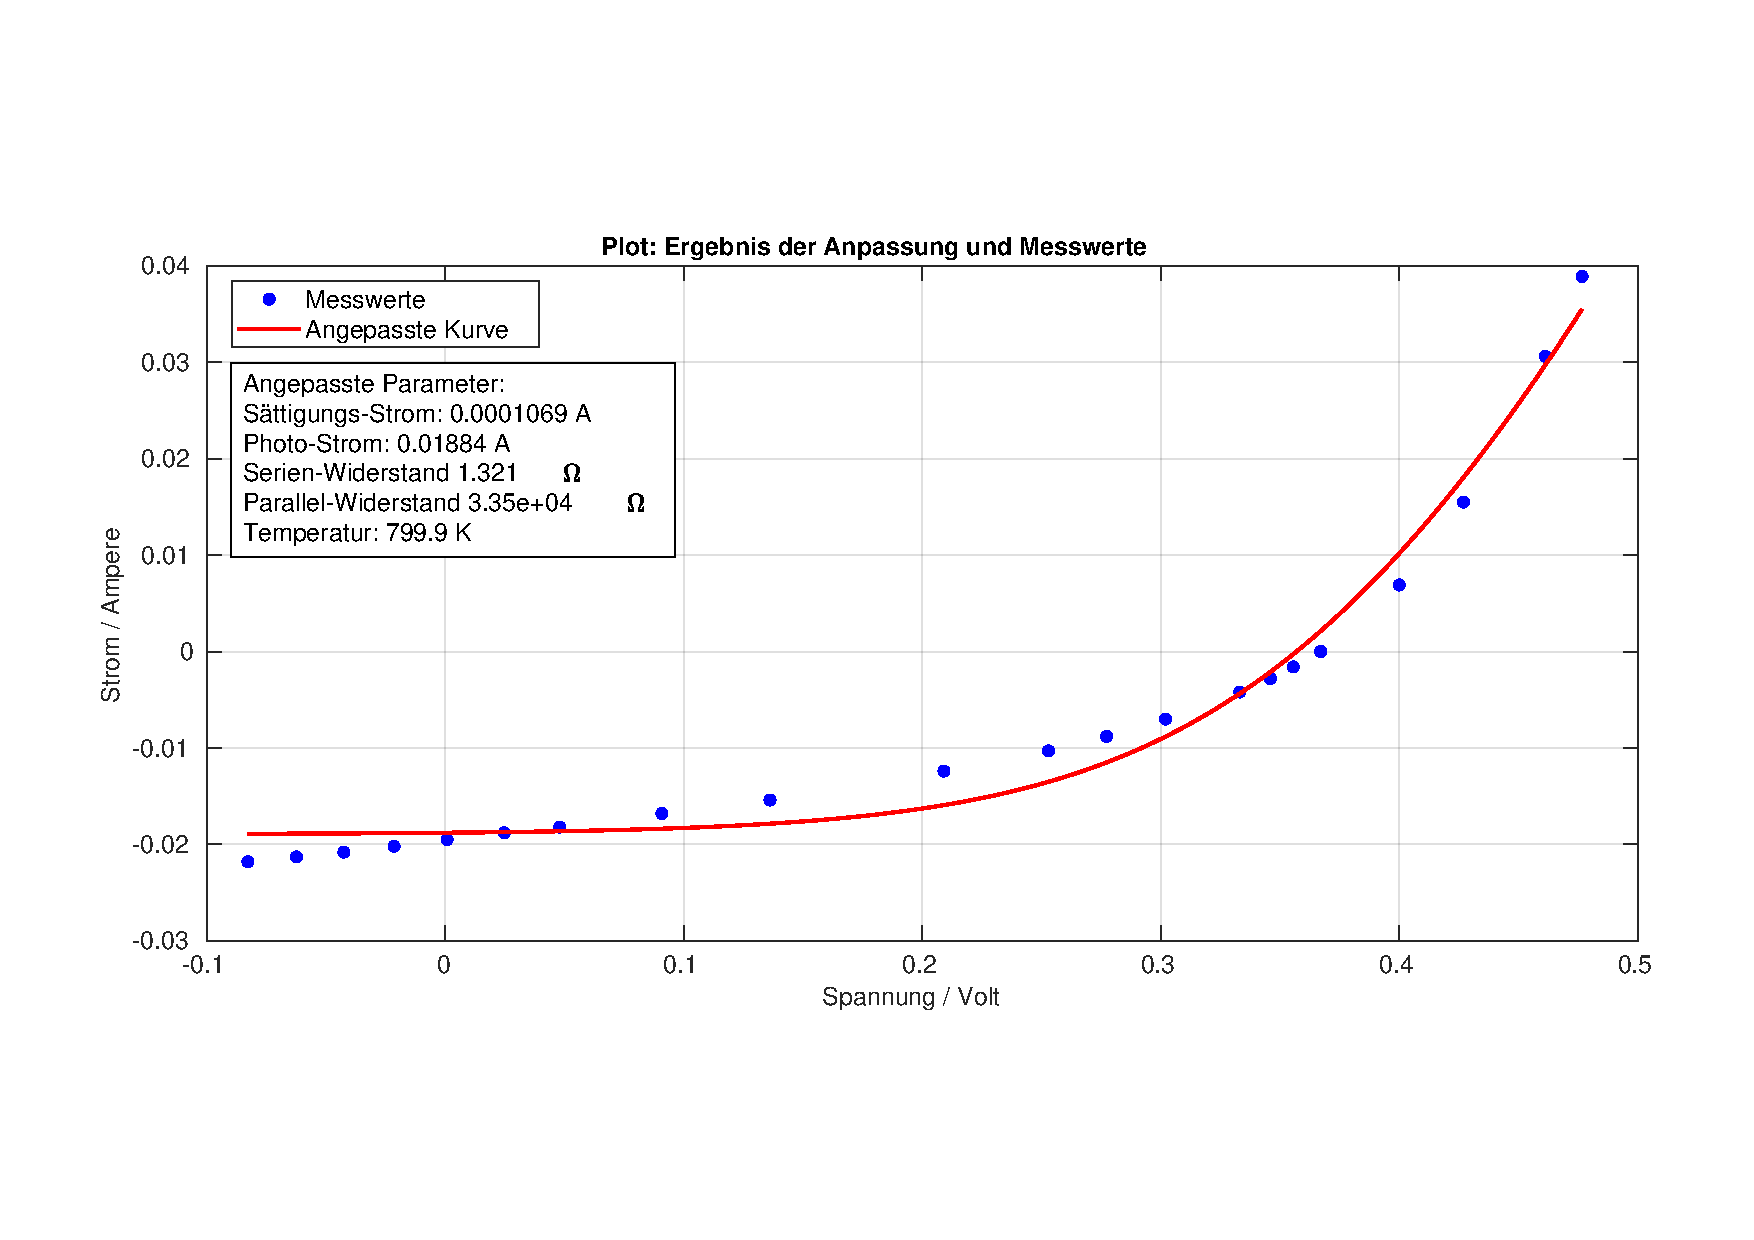
\includegraphics[width = \linewidth]{Bilder/CIS230Plot.pdf}
    \caption{Gefittete Shockley-Gleichung an das CIS-Modul bei 230V Trafospannung}
\end{figure}

\begin{figure}[ht]
    \centering
    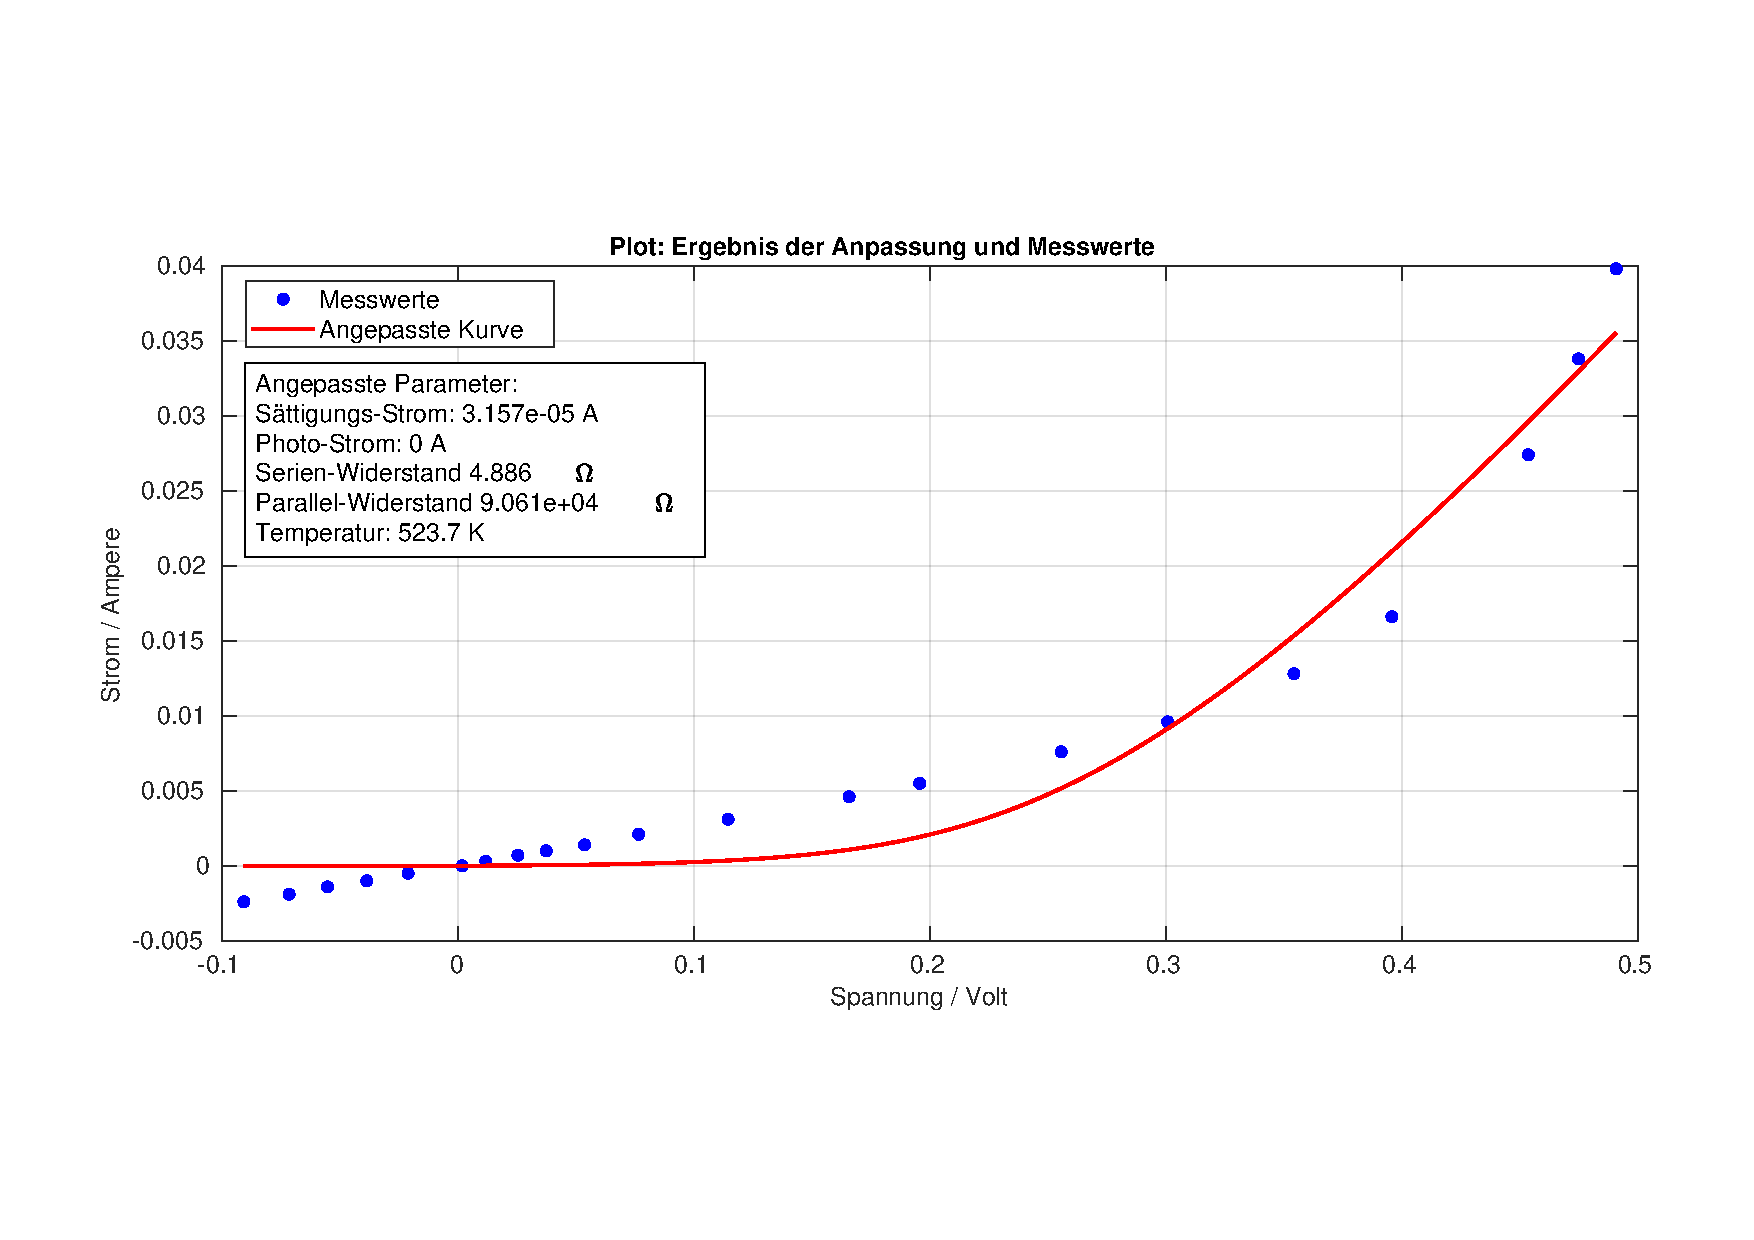
\includegraphics[width = \linewidth]{Bilder/CISDunkelPlot.pdf}
    \caption{Gefittete Schockley-Gleichung an Dunkelmessung der CIS-Zelle}
\end{figure}


\begin{figure}[ht]
    \centering
    \includegraphics[width = \linewidth]{Bilder/SiMonoDunkelPlot.pdf}
    \caption{Gefittete Schockley-Gleichung an das Mono-Si-Modul bei 130V}
\end{figure}
\begin{figure}[ht]
    \centering
    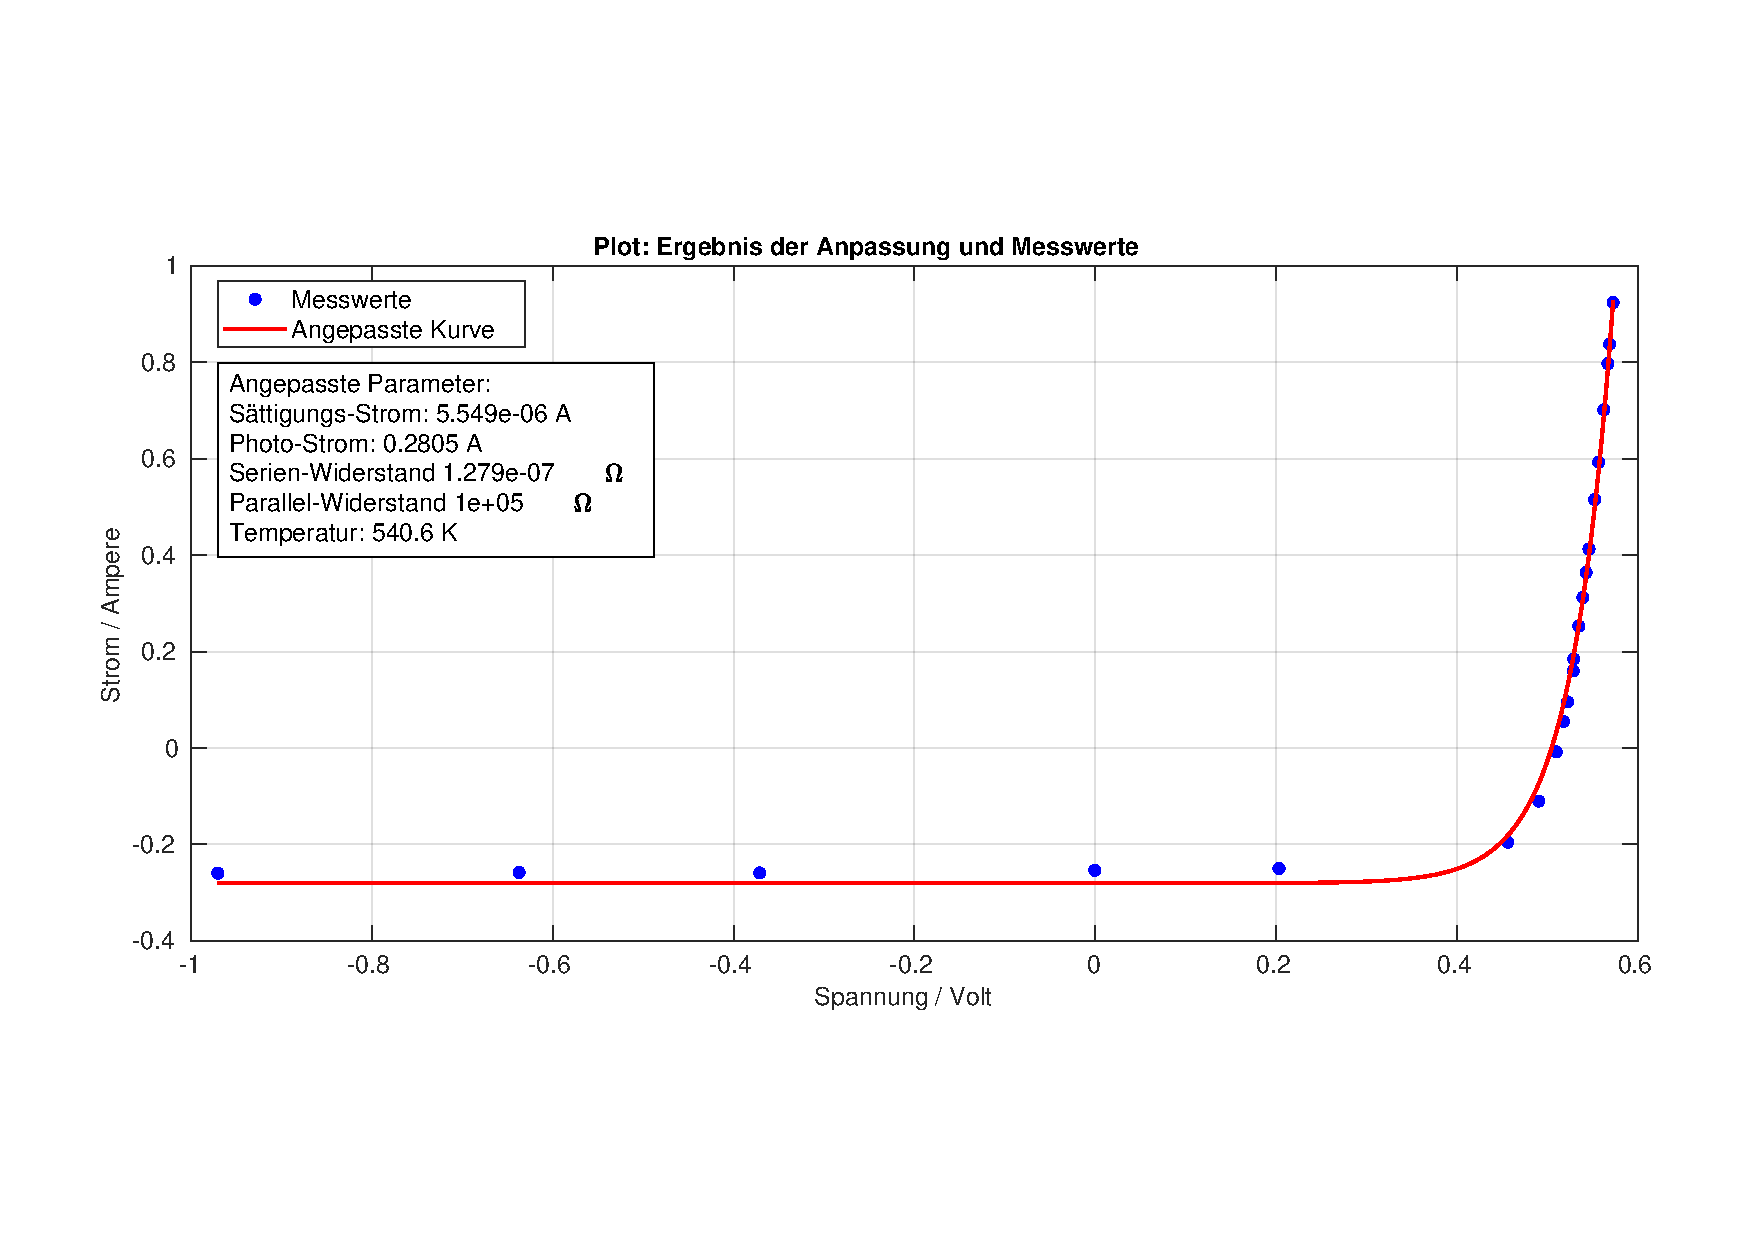
\includegraphics[width = \linewidth]{Bilder/SiMulti130Plot.pdf}
    \caption{Gefittete Schockley-Gleichung an das Mono-Si-Modul bei 130V}
\end{figure}
\begin{figure}[ht]
    \centering
    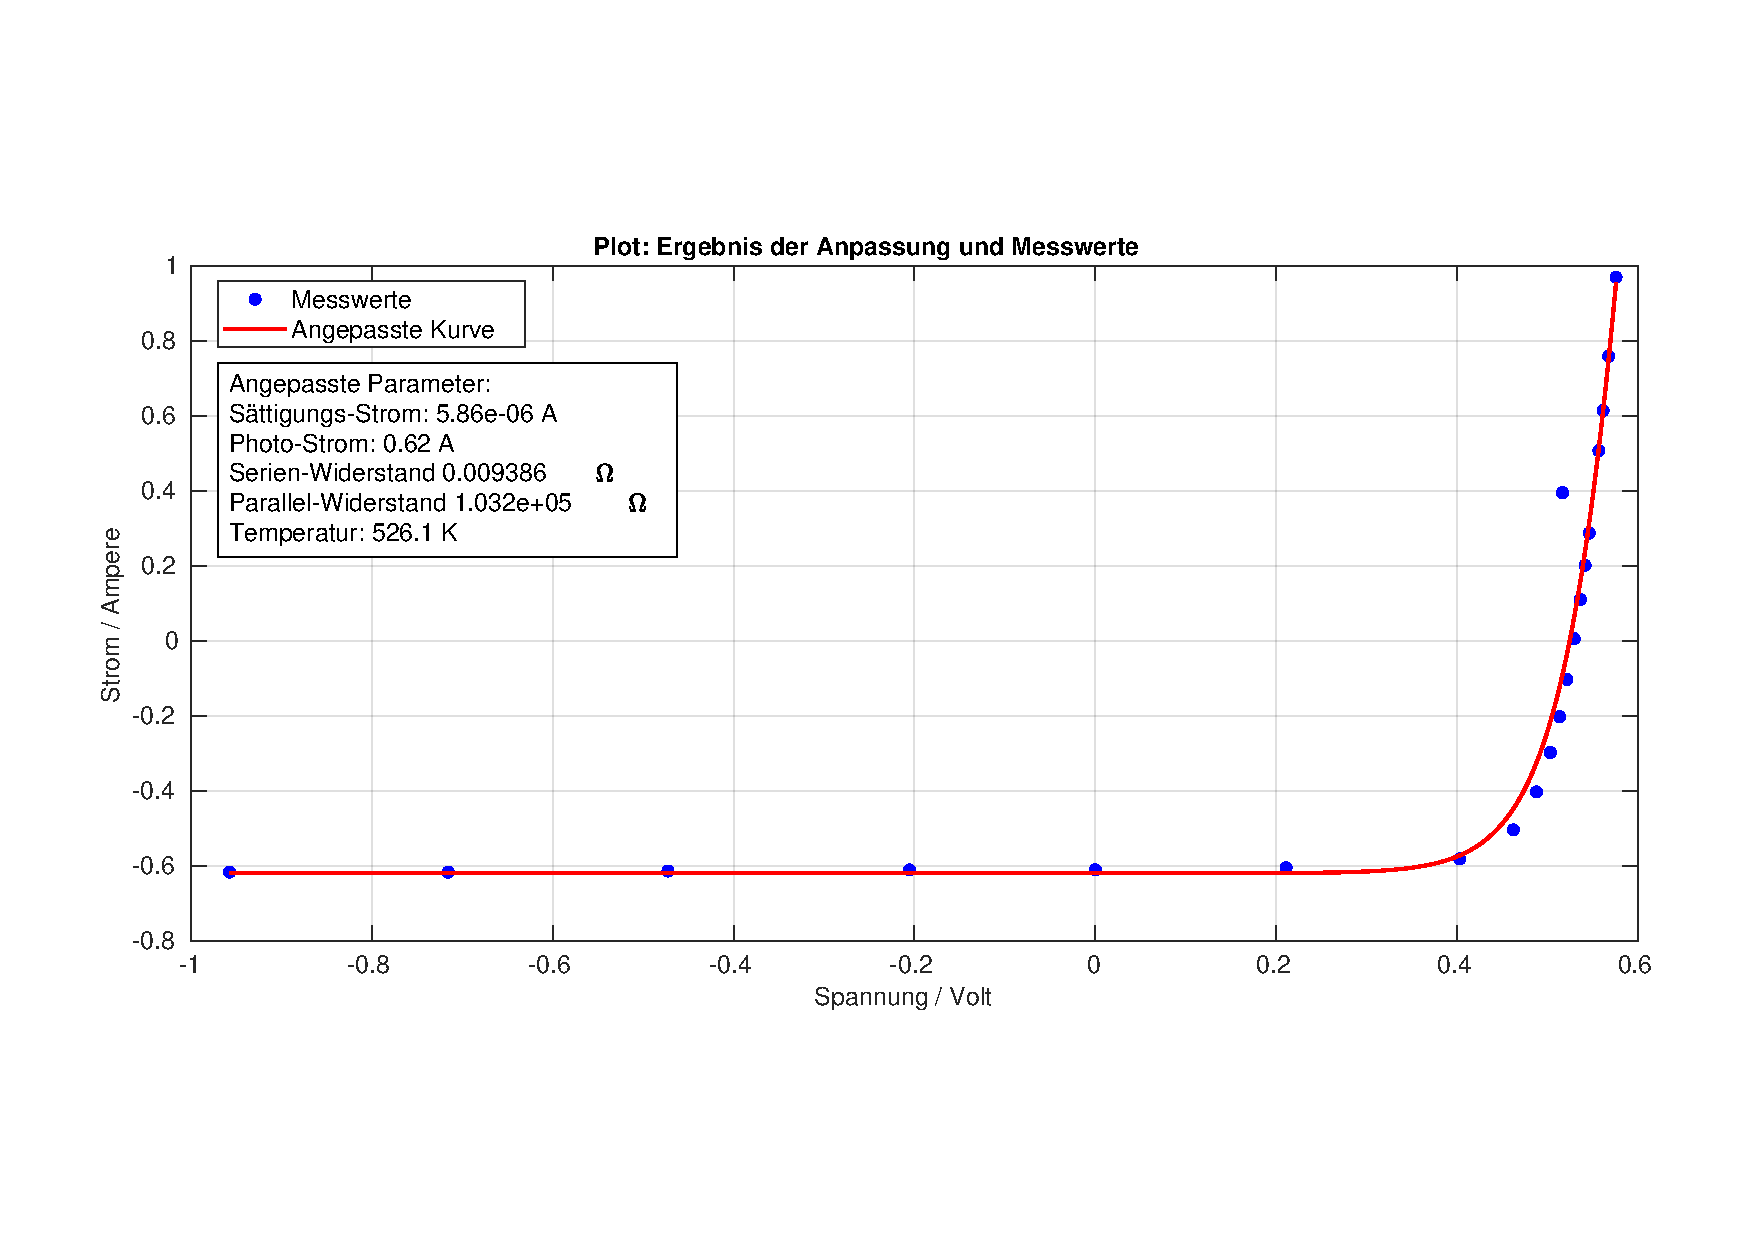
\includegraphics[width = \linewidth]{Bilder/SiMulti180Plot.pdf}
    \caption{Gefittete Schockley-Gleichung an das Mono-Si-Modul bei 130V}
\end{figure}
\begin{figure}[ht]
    \centering
    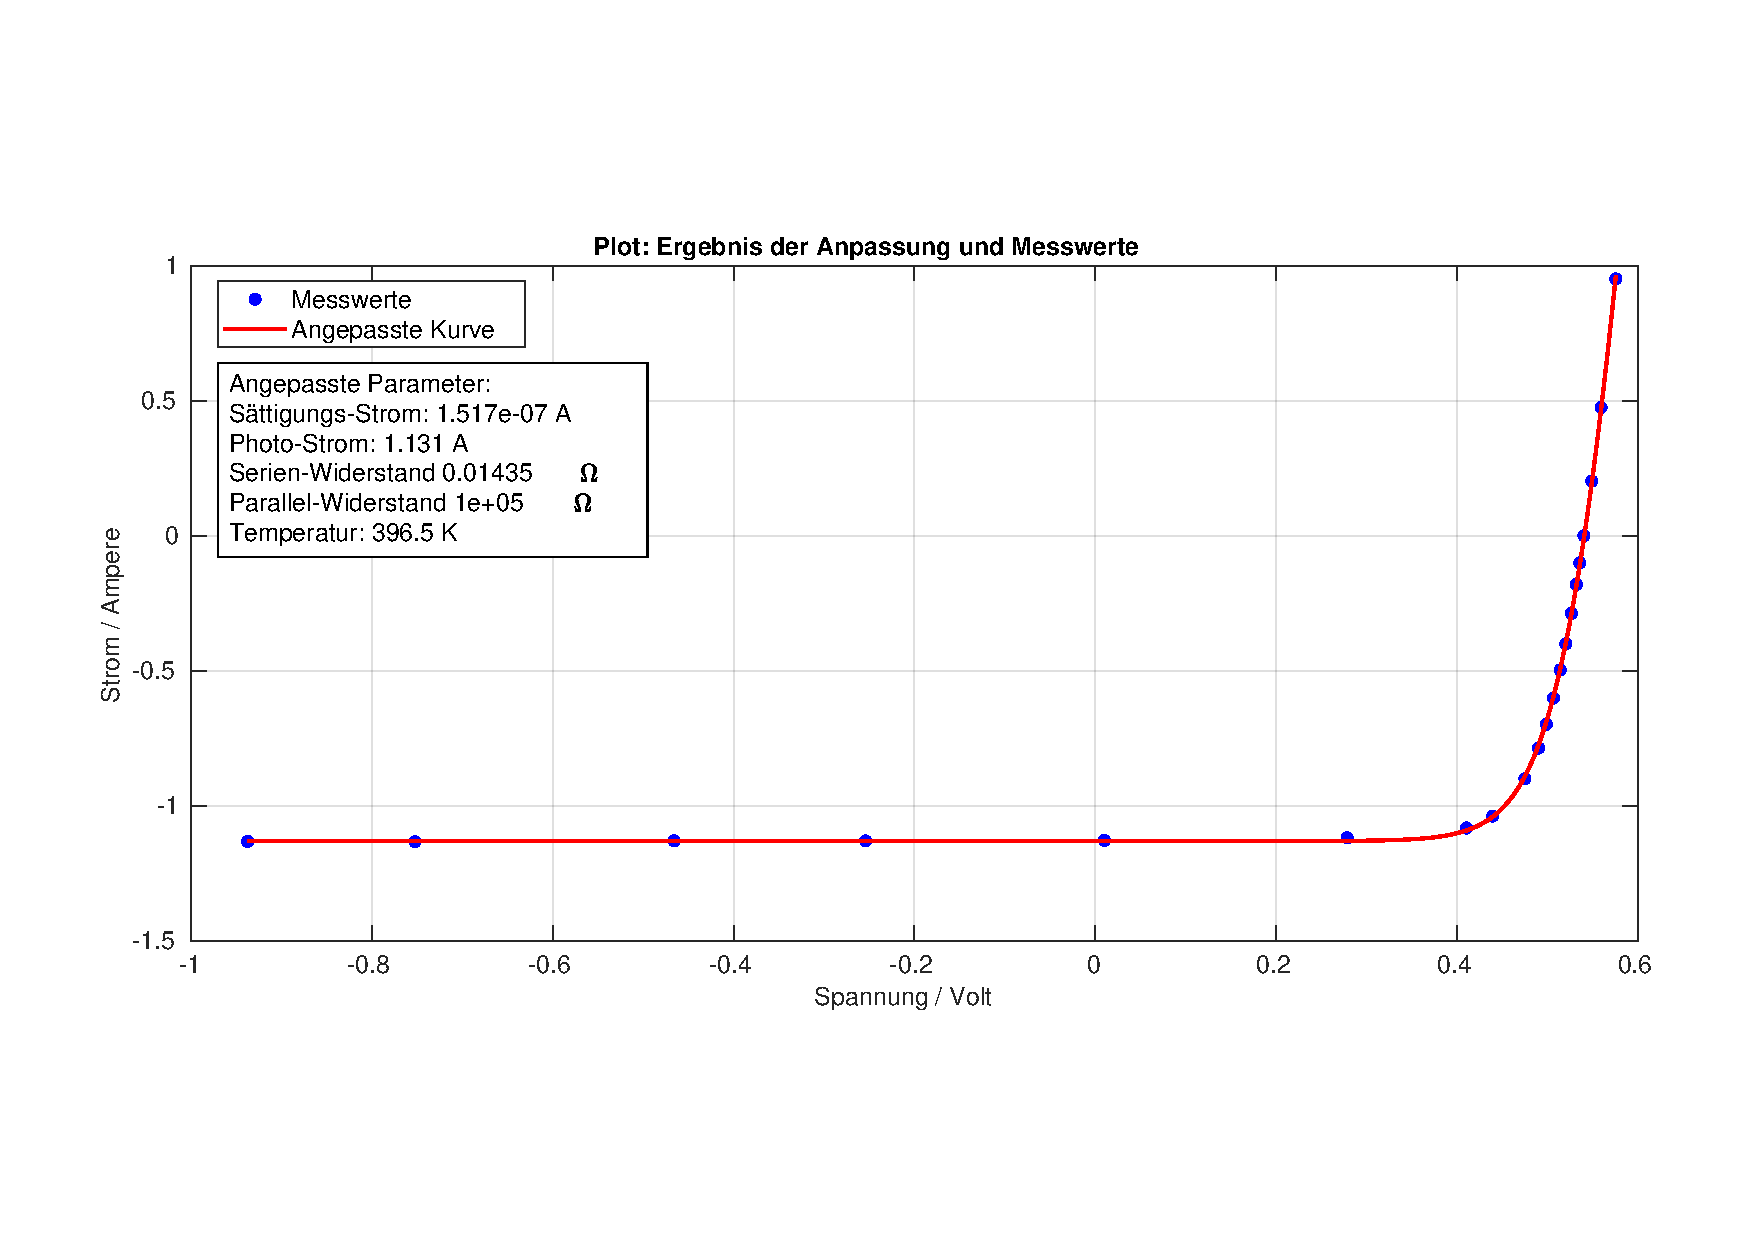
\includegraphics[width = \linewidth]{Bilder/SiMulti230Plot.pdf}
    \caption{Gefittete Schockley-Gleichung an das Mono-Si-Modul bei 130V}
\end{figure}
\begin{figure}[ht]
    \centering
    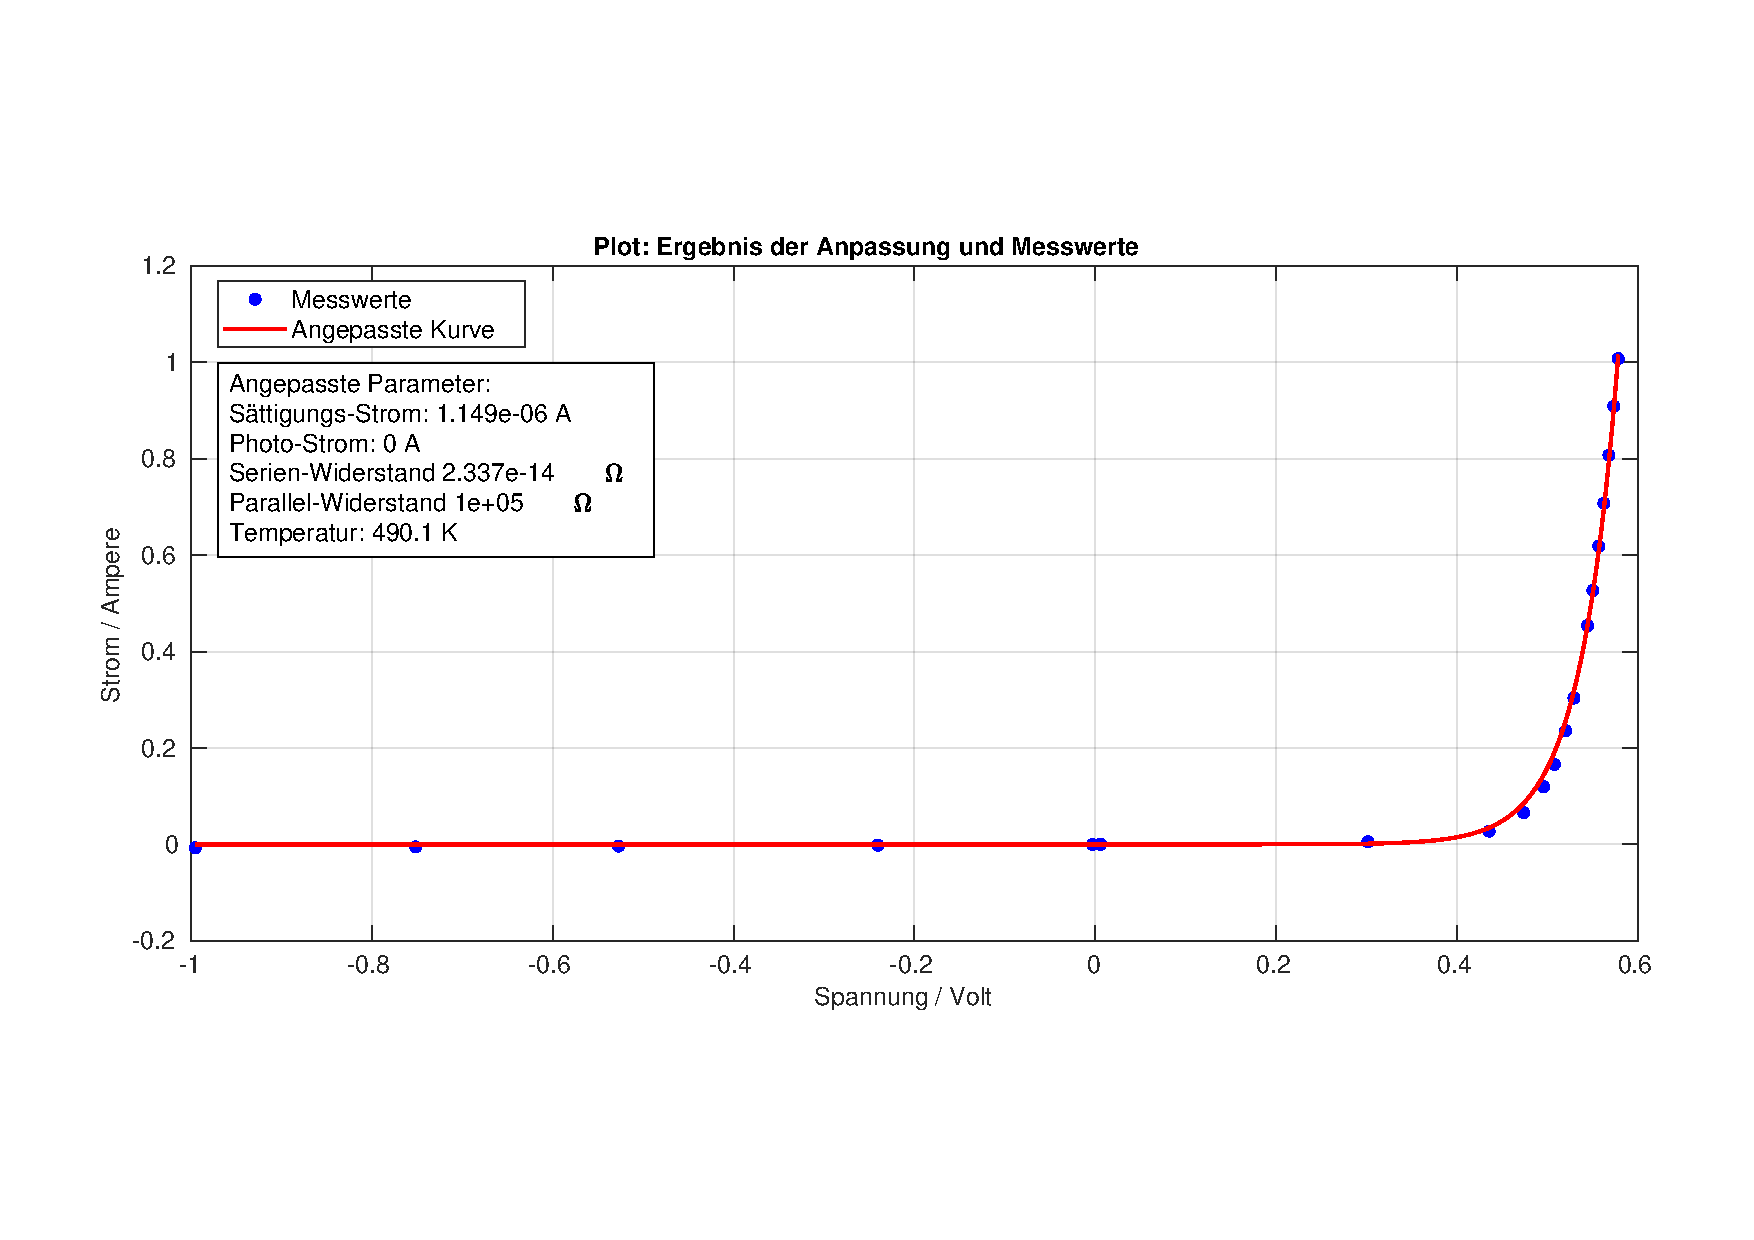
\includegraphics[width = \linewidth]{Bilder/SiMultiDunkelPlot.pdf}
    \caption{Gefittete Schockley-Gleichung an das Mono-Si-Modul bei 130V}
\end{figure}
\clearpage


\section{Wirkungsgrad}
\label{section:AnhangWirkungsgrad}

\begin{figure}[ht]
    \centering
    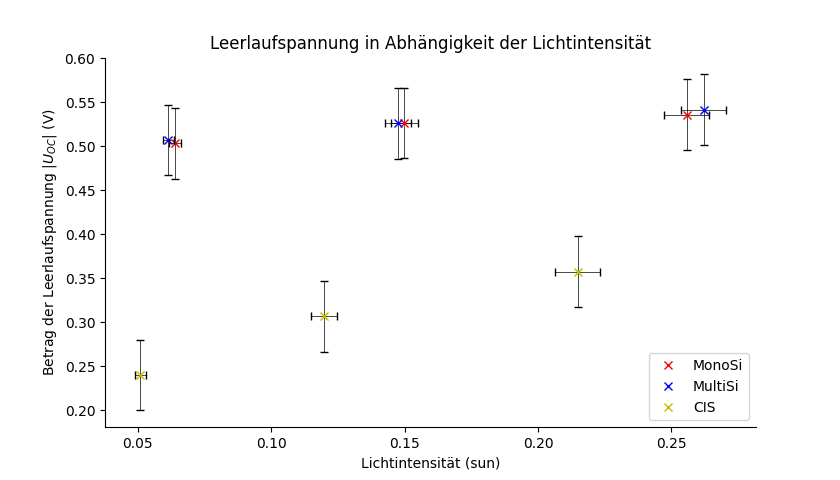
\includegraphics[width = \linewidth]{Bilder/UOCInt.png}
    \caption{Leerlaufspannung in Abhängigkeit der Lichtintensität bei drei unterschiedlichen Solarmodule. Die Fehler 
    sind aus Schwankungen geschätzt}
\end{figure}

\begin{figure}[ht]
    \centering
    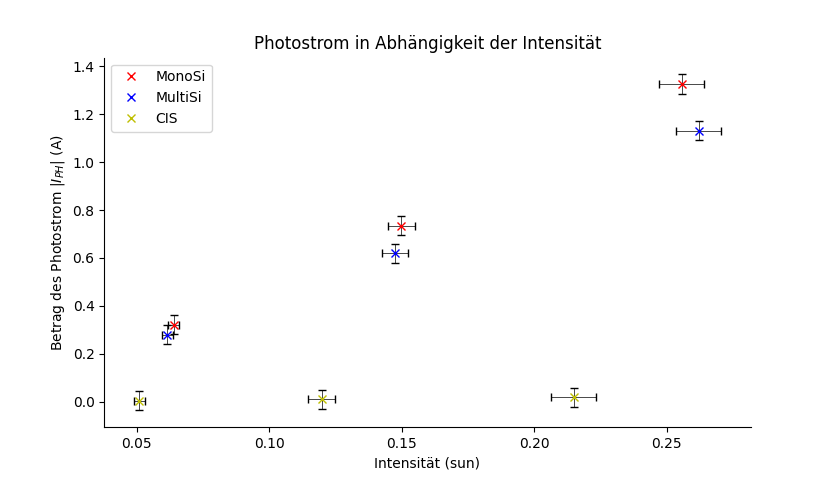
\includegraphics[width = \linewidth]{Bilder/IPhInt.png}
    \caption{Photostrom in Abhängigkeit der Lichtintensität bei drei unterschiedlichen Solarmodule. Die Fehler 
    sind aus Schwankungen geschätzt}

\end{figure}

\begin{figure}[ht]
    \centering
    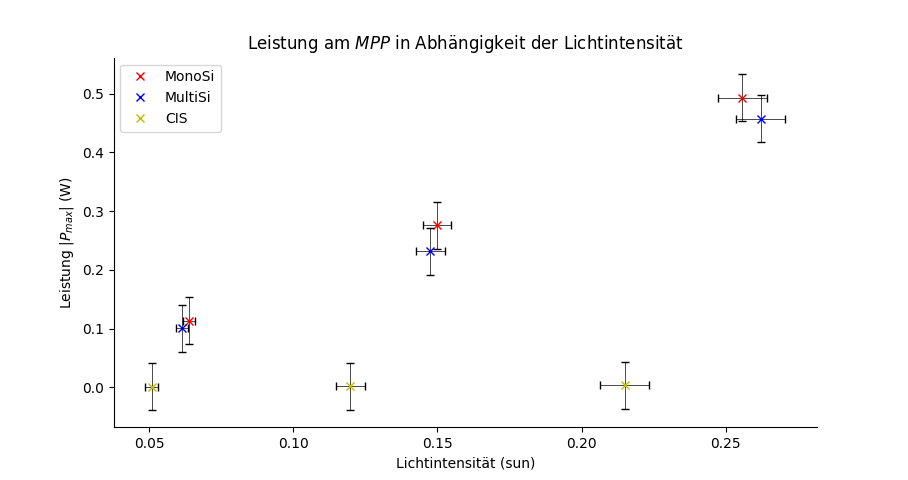
\includegraphics[width = \linewidth]{Bilder/MPPInt.png}
    \caption{Maximale Leistung $P_{Max}$ in Abhängigkeit der Lichtintensität bei drei unterschiedlichen Solarmodule. Die Fehler 
    sind aus Schwankungen geschätzt}  
\end{figure}

\begin{figure}[ht]
    \centering
    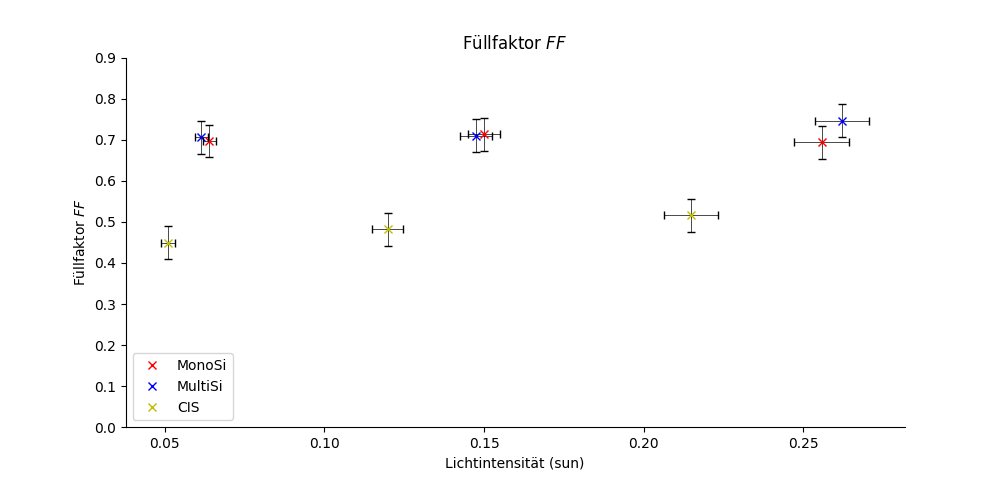
\includegraphics[width = \linewidth]{Bilder/FFInt.png}
    \caption{Füllfaktor $FF$ in Abhängigkeit der Lichtintensität bei drei unterschiedlichen Solarmodule. Die Fehler 
    sind aus Schwankungen geschätzt}  
\end{figure}

\clearpage
\subsection{Messdaten}
\begin{figure}[h]
    \captionsetup{justification=centering,margin=2cm}
    \centering
    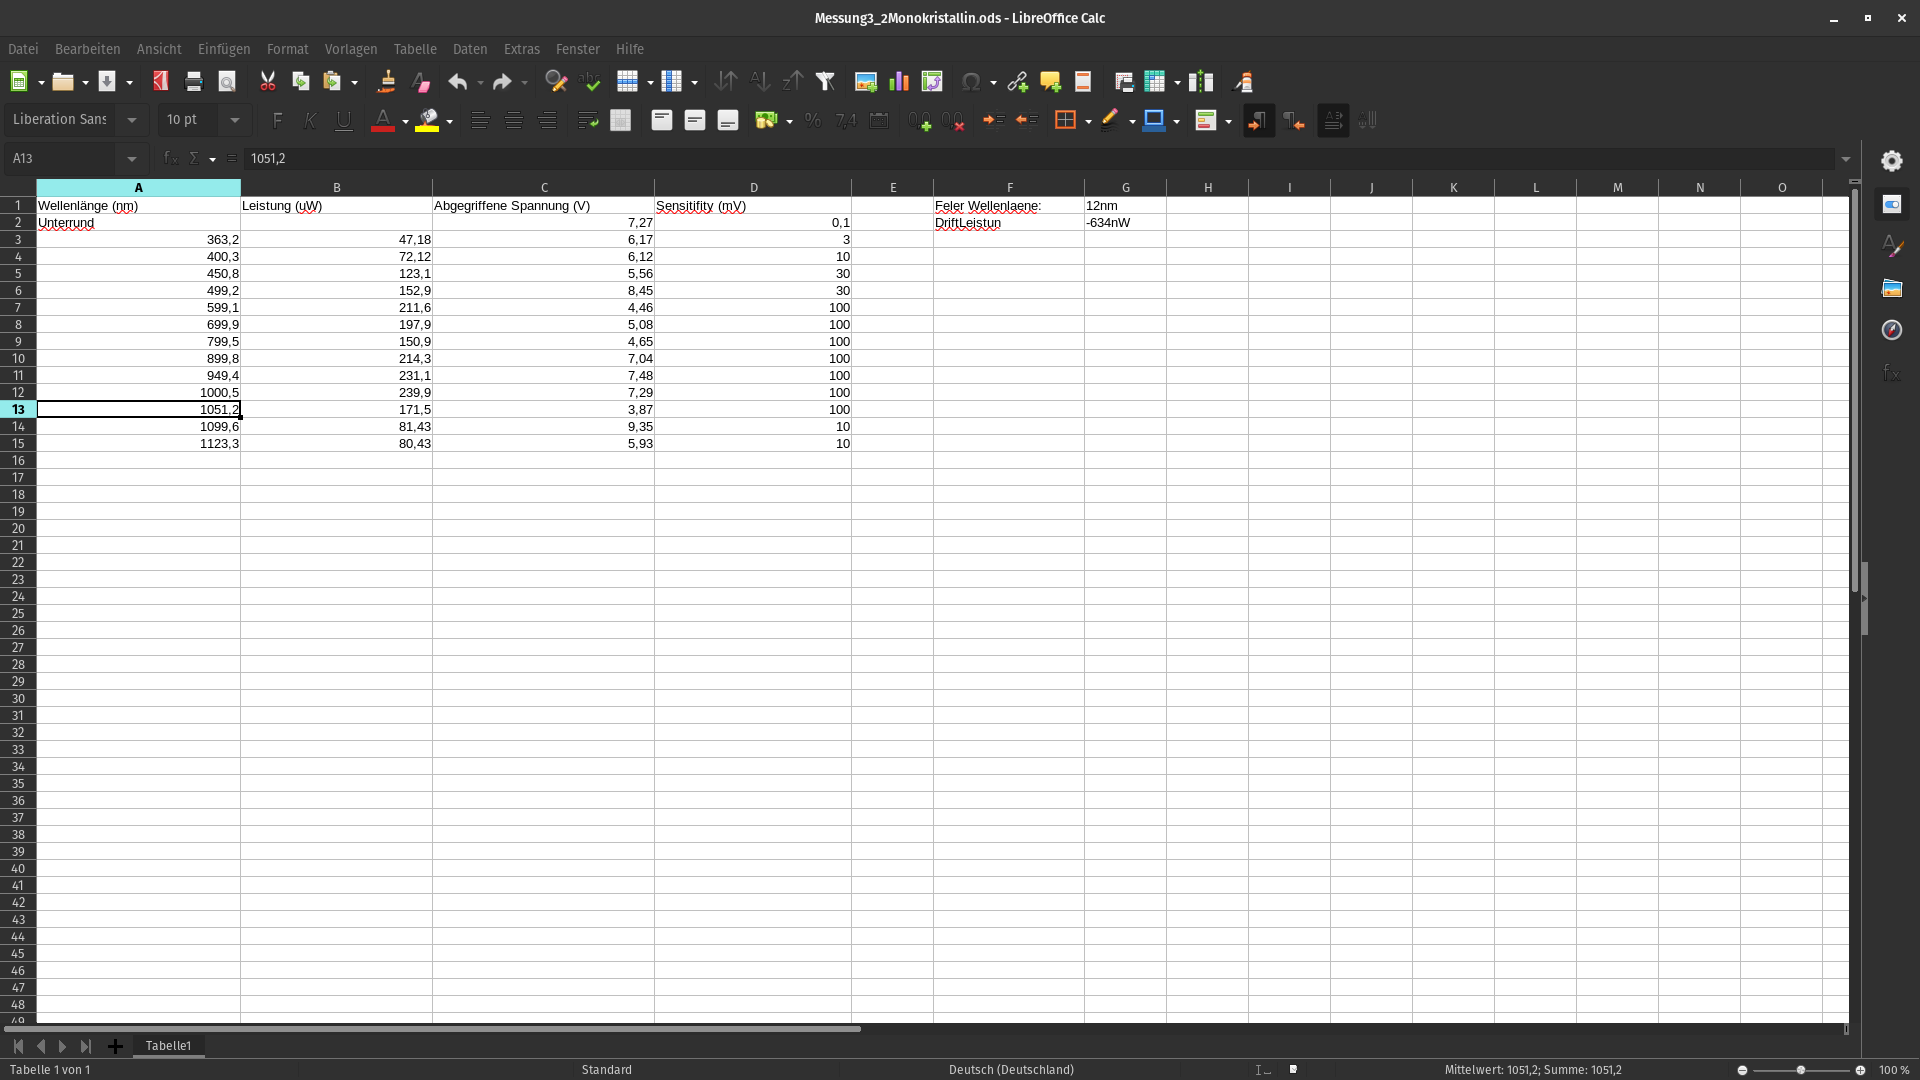
\includegraphics[angle = 90, width = 12cm]{Bilder/Daten/MessunngMonoSI.png}
    \caption{Messdaten zur Messung der spektralen Empfindlichkeit der MonoSi-Zelle}
\end{figure}


\begin{figure}[h]
    \captionsetup{justification=centering,margin=2cm}
    \centering
    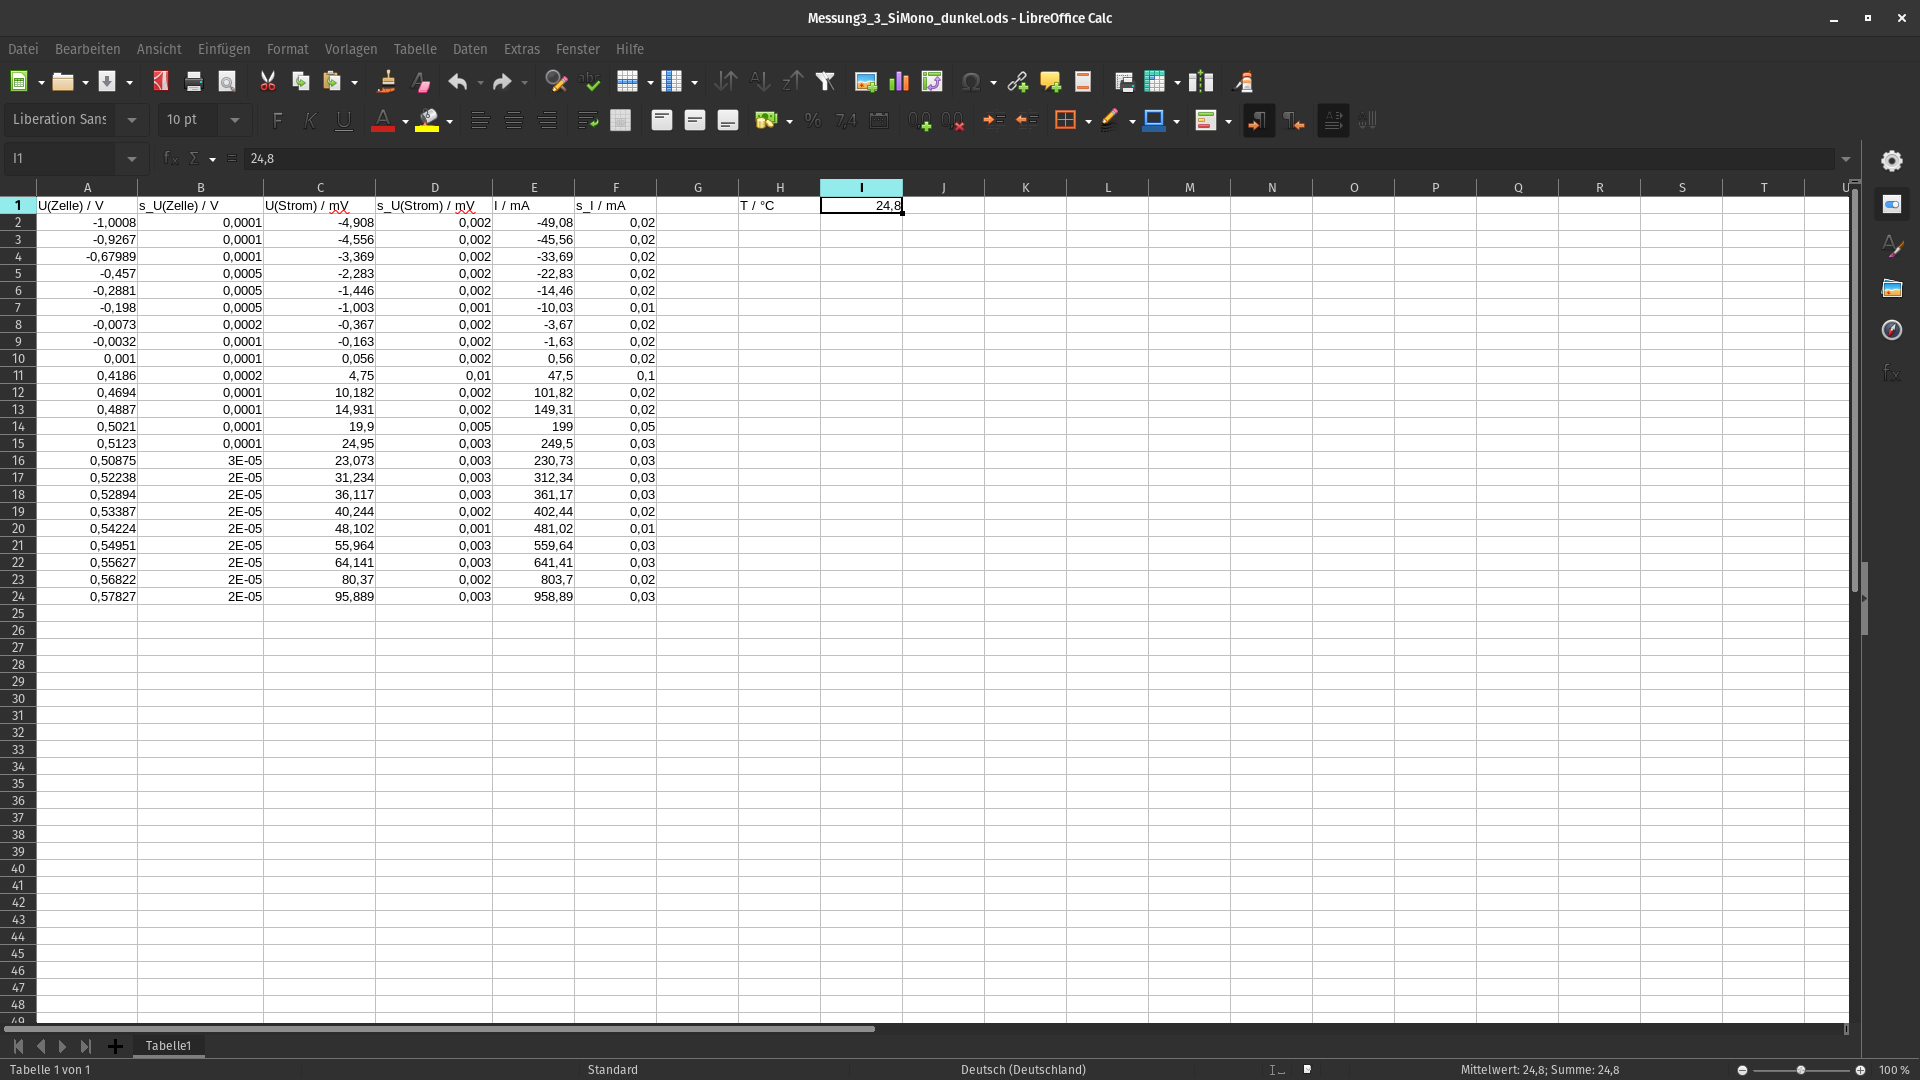
\includegraphics[angle = 90, width = 12cm]{Bilder/Daten/MessunngMonoSiDunkel.png}
    \caption{Dunkelmessung der MonoSi-Zelle}
\end{figure}

\begin{figure}[h]
    \captionsetup{justification=centering,margin=2cm}
    \centering
    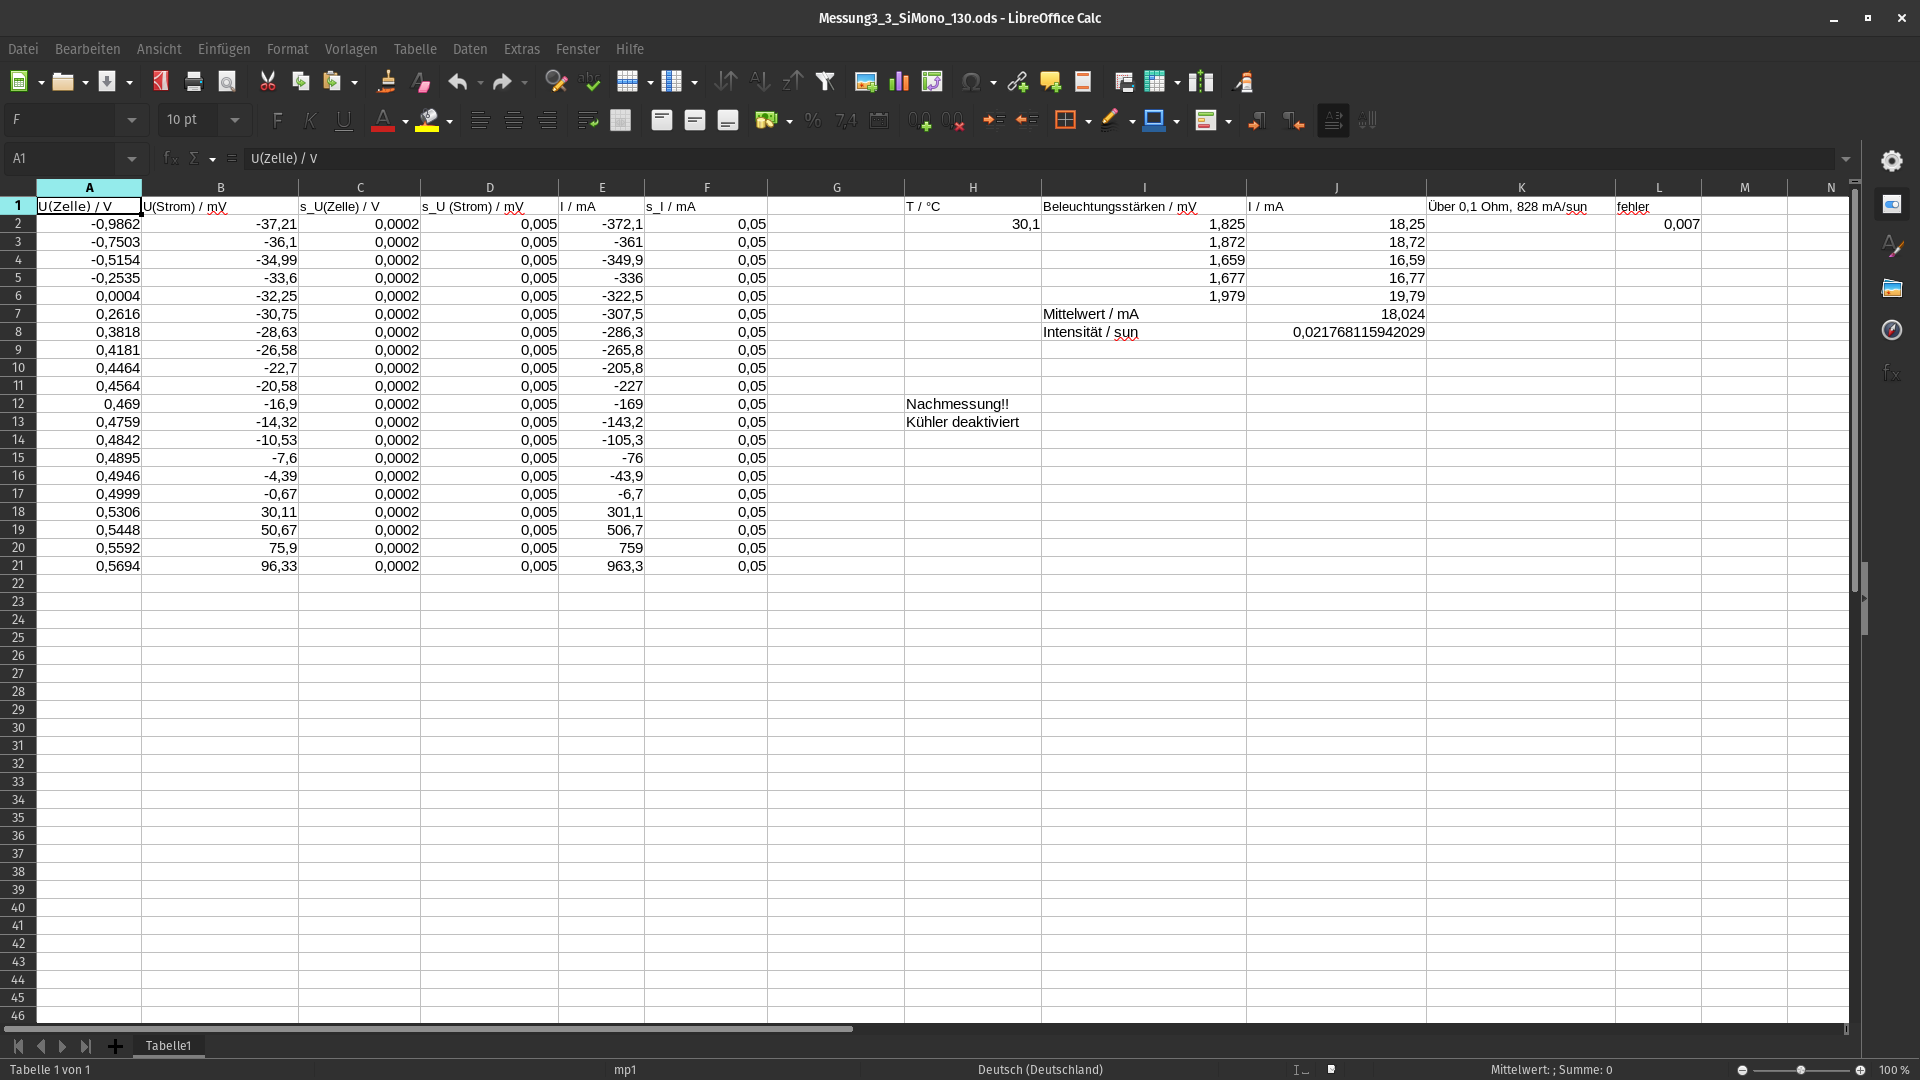
\includegraphics[angle = 90, width = 12cm]{Bilder/Daten/MessunngMonoSi130.png}
    \caption{Beleuchtete Messung bei 130V am Stelltransformator}
\end{figure}

\begin{figure}[h]
    \captionsetup{justification=centering,margin=2cm}
    \centering
    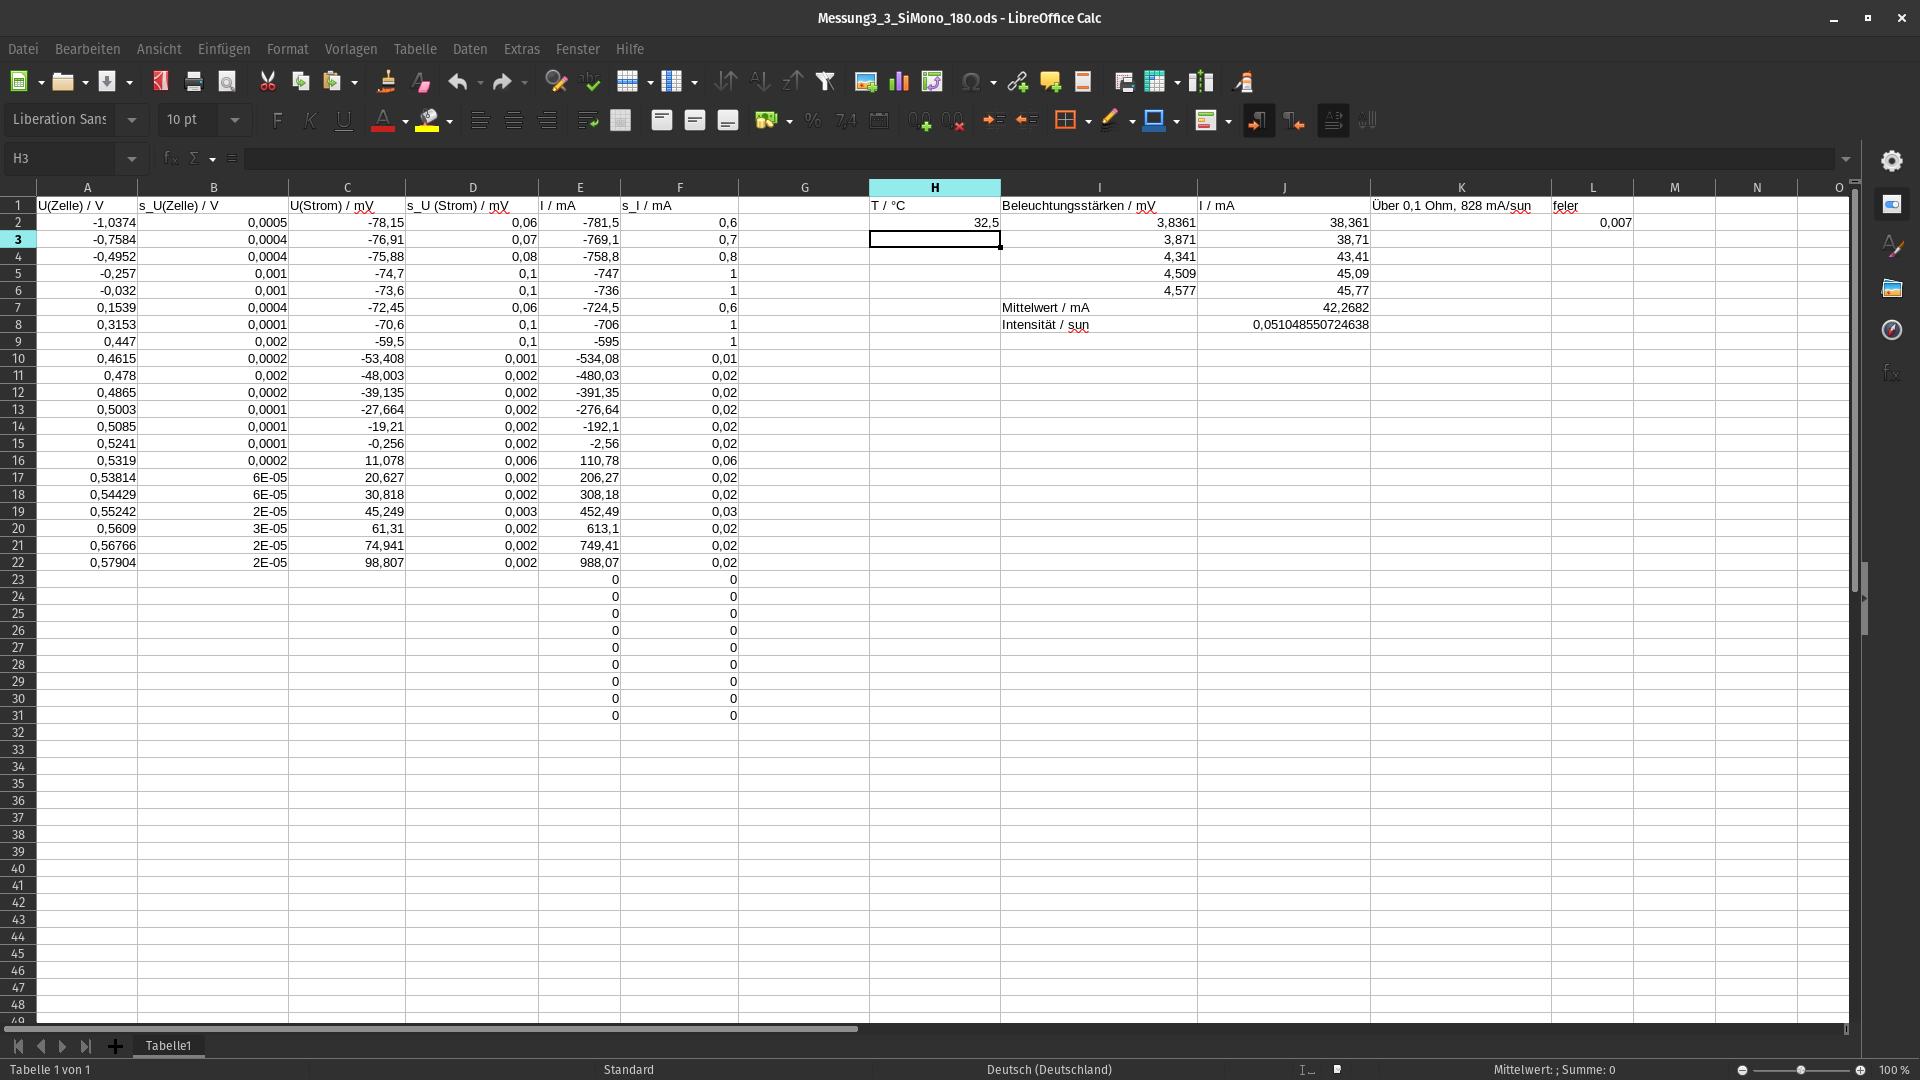
\includegraphics[angle = 90, width = 12cm]{Bilder/Daten/MessunngMonoSi180.png}
    \caption{Beleuchtete Messung bei 180V am Stelltransformator}
\end{figure}

\begin{figure}[h]
    \captionsetup{justification=centering,margin=2cm}
    \centering
    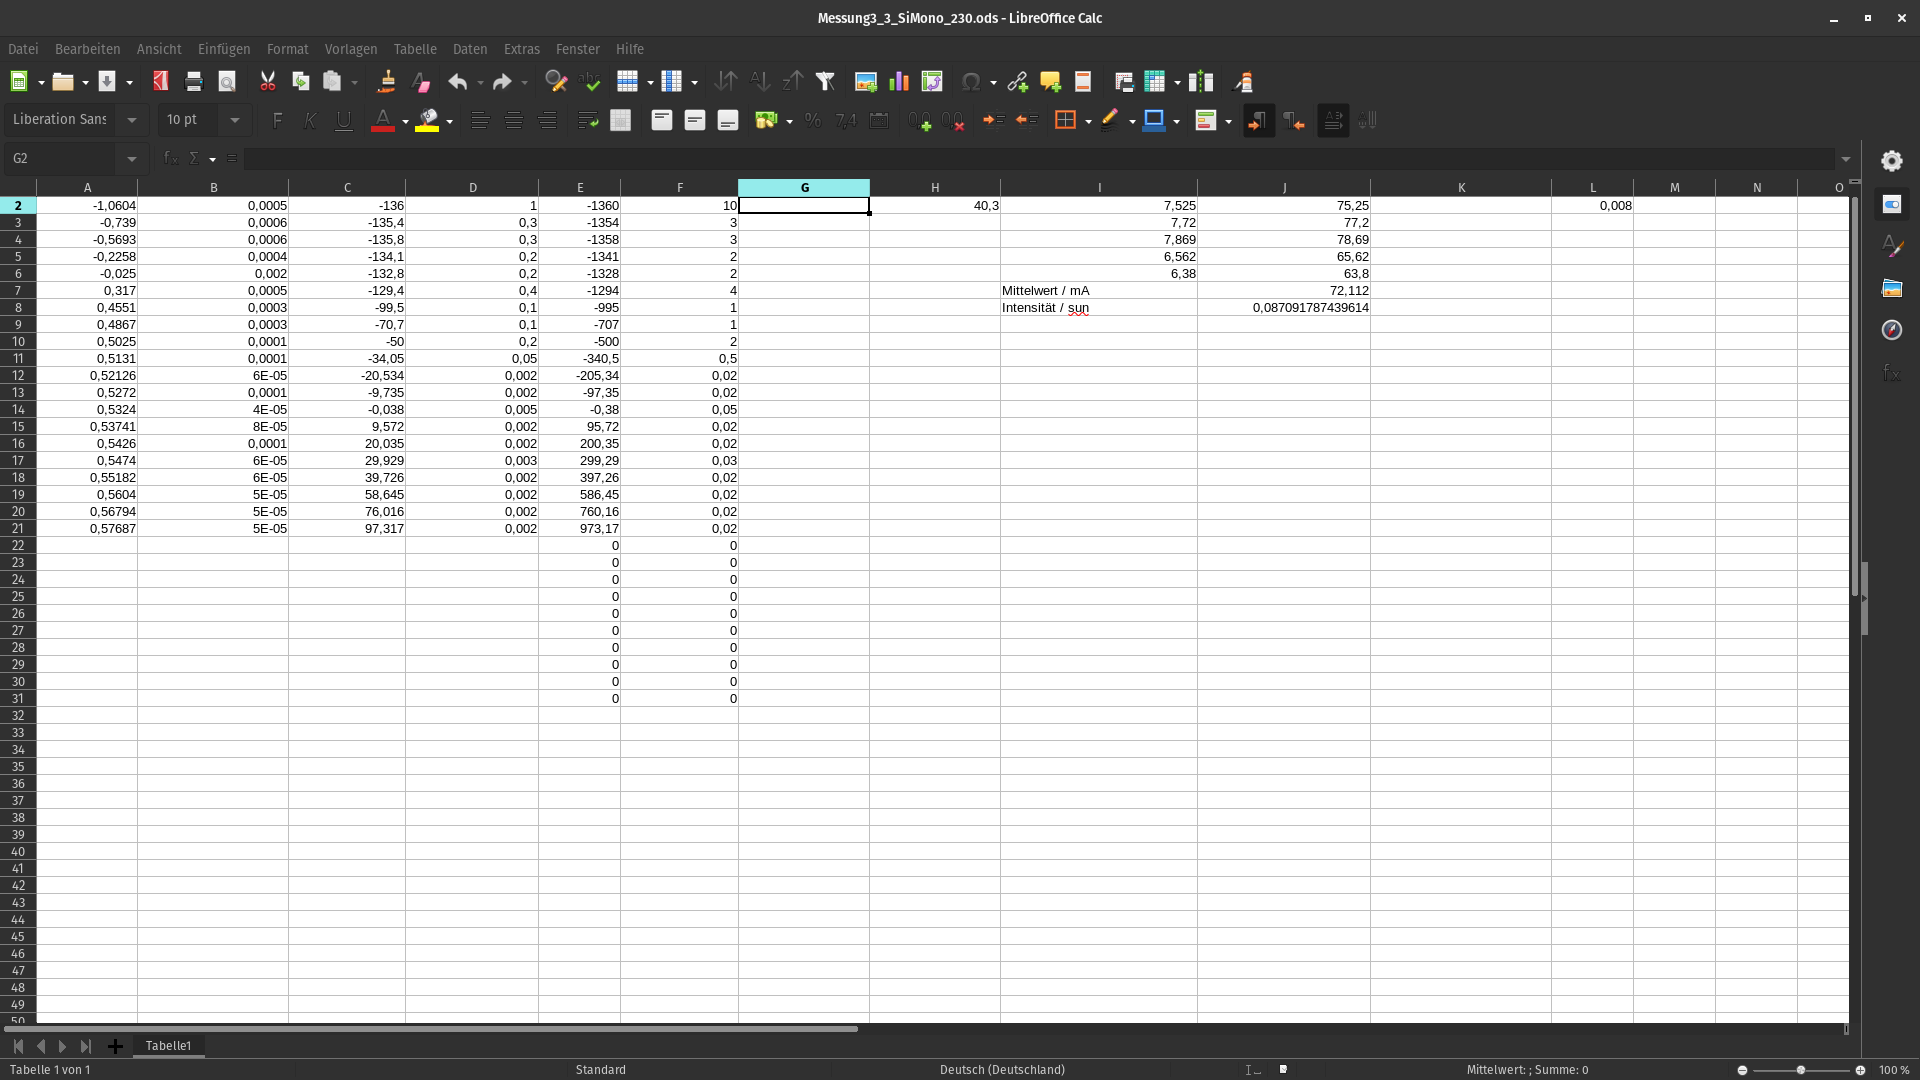
\includegraphics[angle = 90, width = 12cm]{Bilder/Daten/MessungMonoSi230.png}
    \caption{Beleuchtete Messung bei 230V am Stelltransformator}
\end{figure}






\begin{figure}[h]
    \captionsetup{justification=centering,margin=2cm}
    \centering
    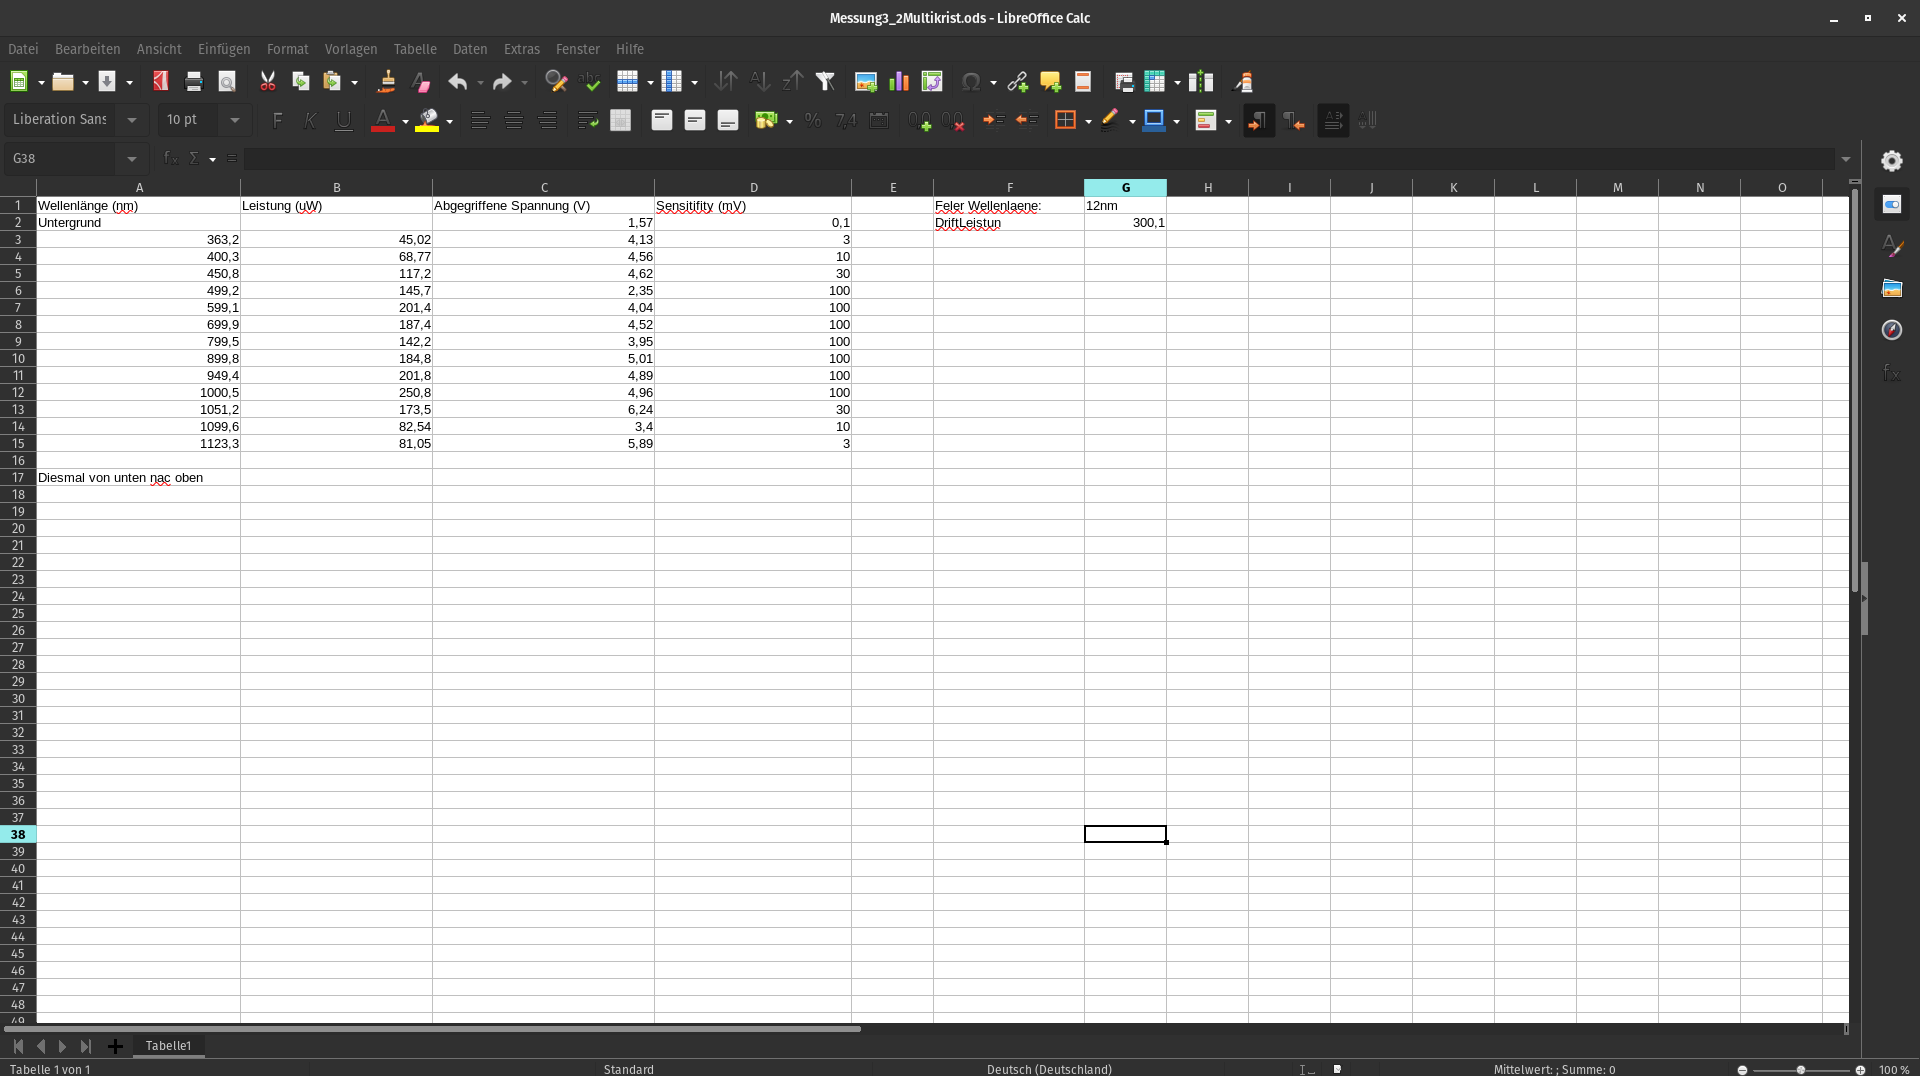
\includegraphics[angle = 90, width = 12cm]{Bilder/Daten/MessunngMultiSi.png}
    \caption{Messdaten zur Messung der spektralen Empfindlichkeit der MultiSi-Zelle}
\end{figure}


\begin{figure}[h]
    \captionsetup{justification=centering,margin=2cm}
    \centering
    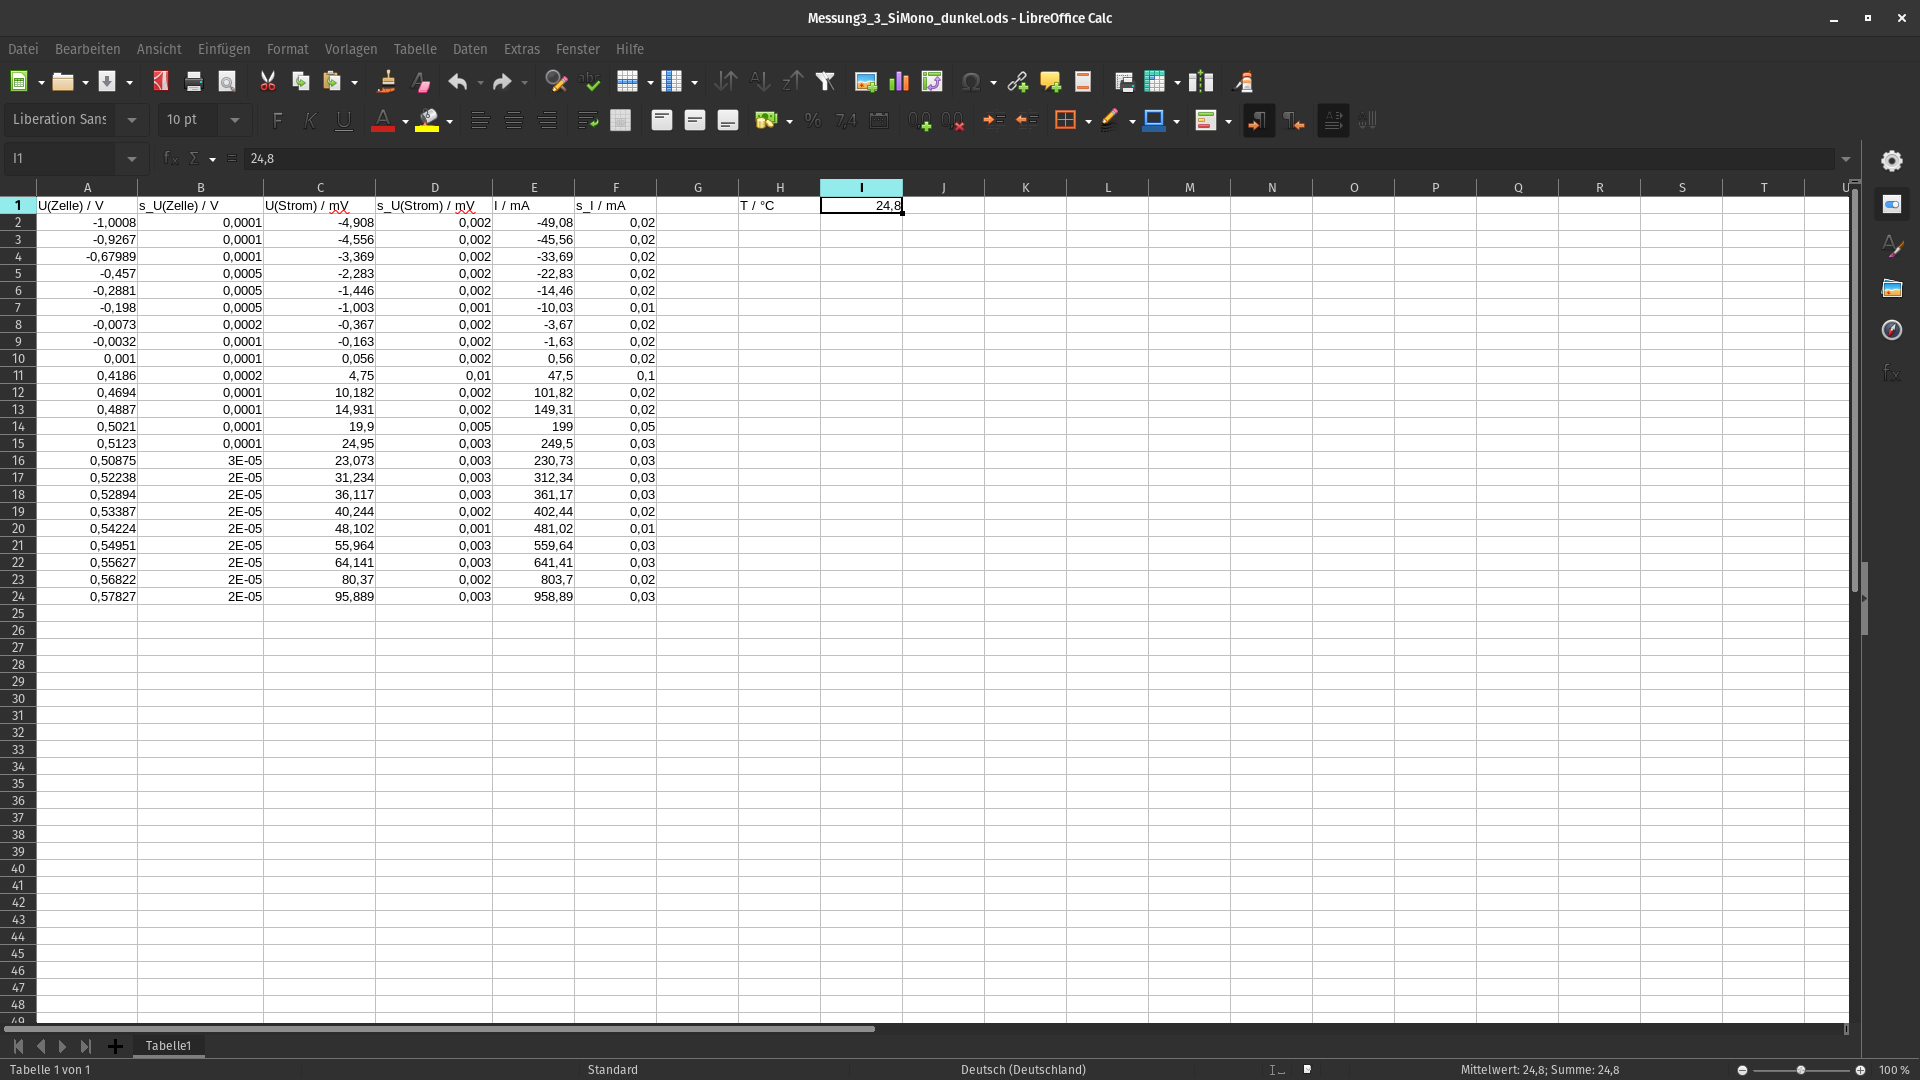
\includegraphics[angle = 90, width = 12cm]{Bilder/Daten/MessunngMonoSiDunkel.png}
    \caption{Dunkelmessung der MultiSi-Zelle}
\end{figure}

\begin{figure}[h]
    \captionsetup{justification=centering,margin=2cm}
    \centering
    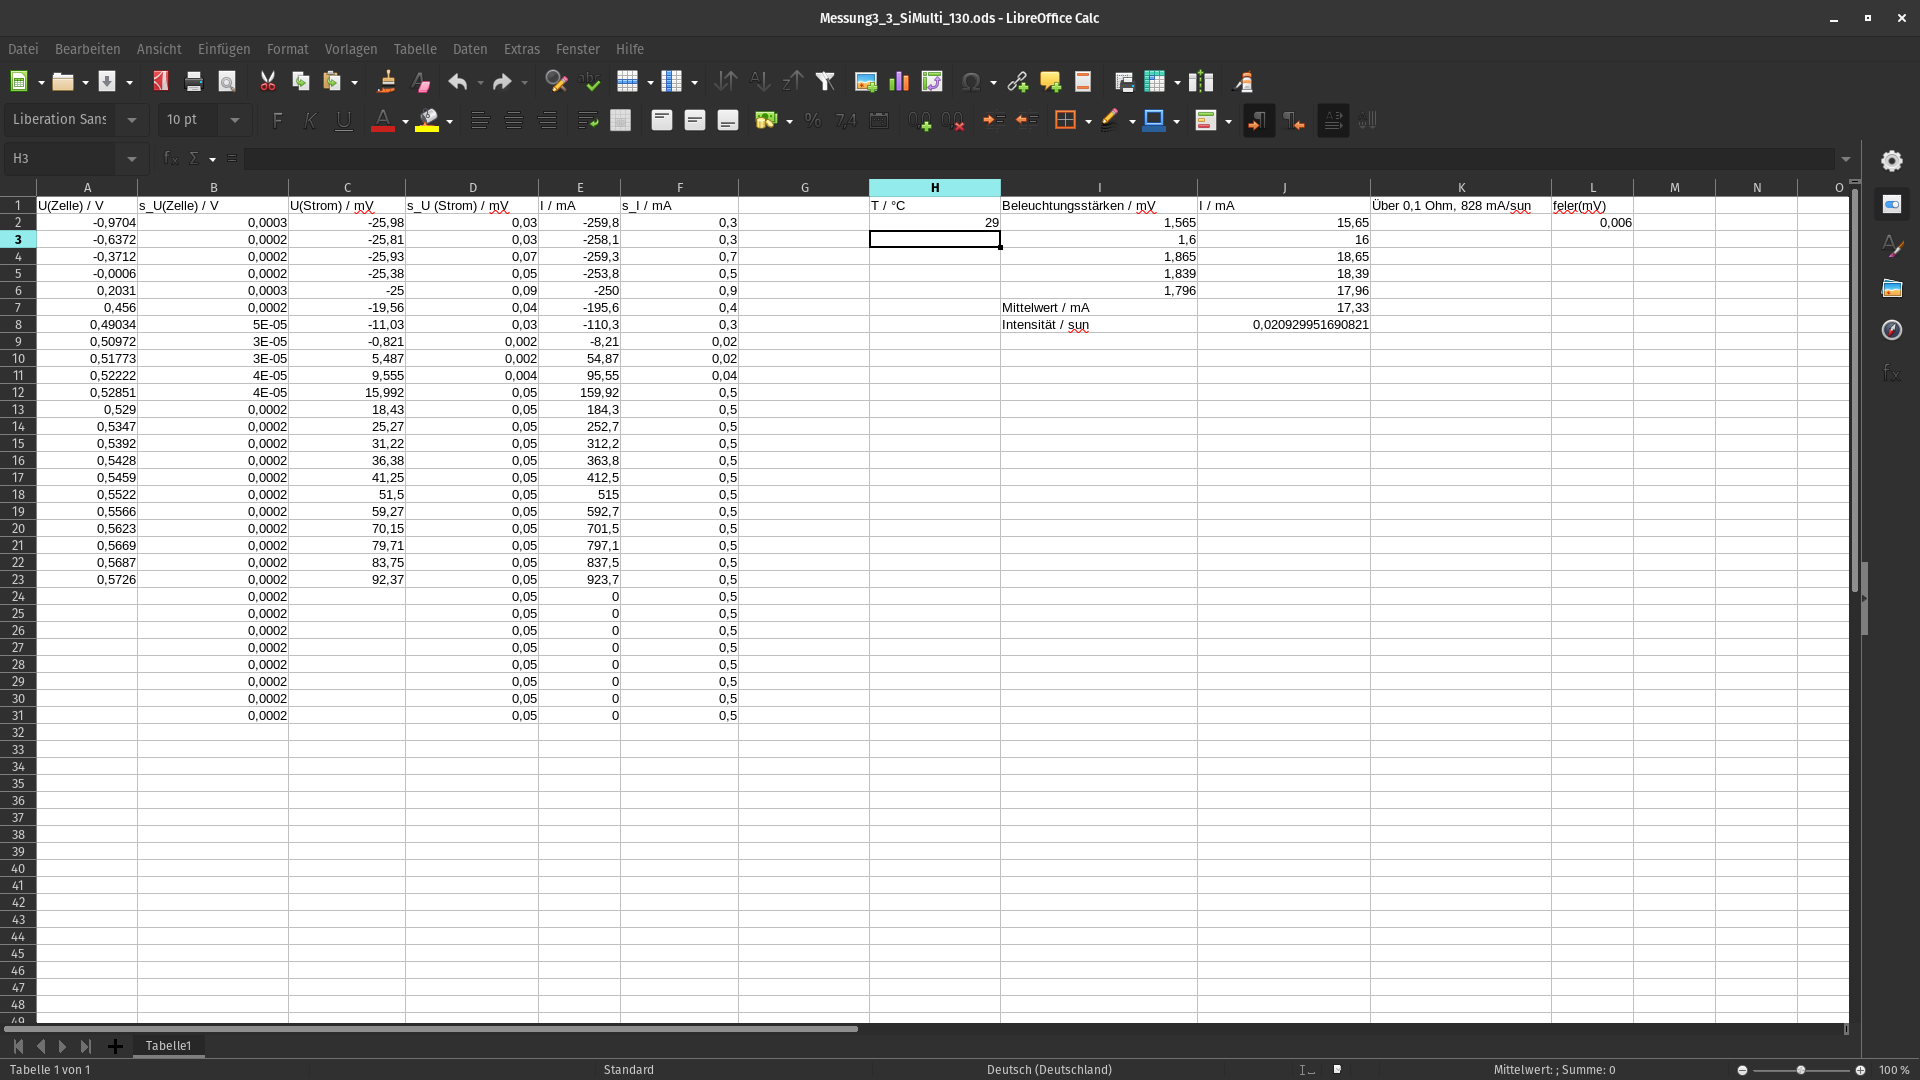
\includegraphics[angle = 90, width = 12cm]{Bilder/Daten/MessunngMulriSi130.png}
    \caption{Beleuchtete Messung bei 130V am Stelltransformator an der Multi-Si-Zelle}
\end{figure}

\begin{figure}[h]
    \captionsetup{justification=centering,margin=2cm}
    \centering
    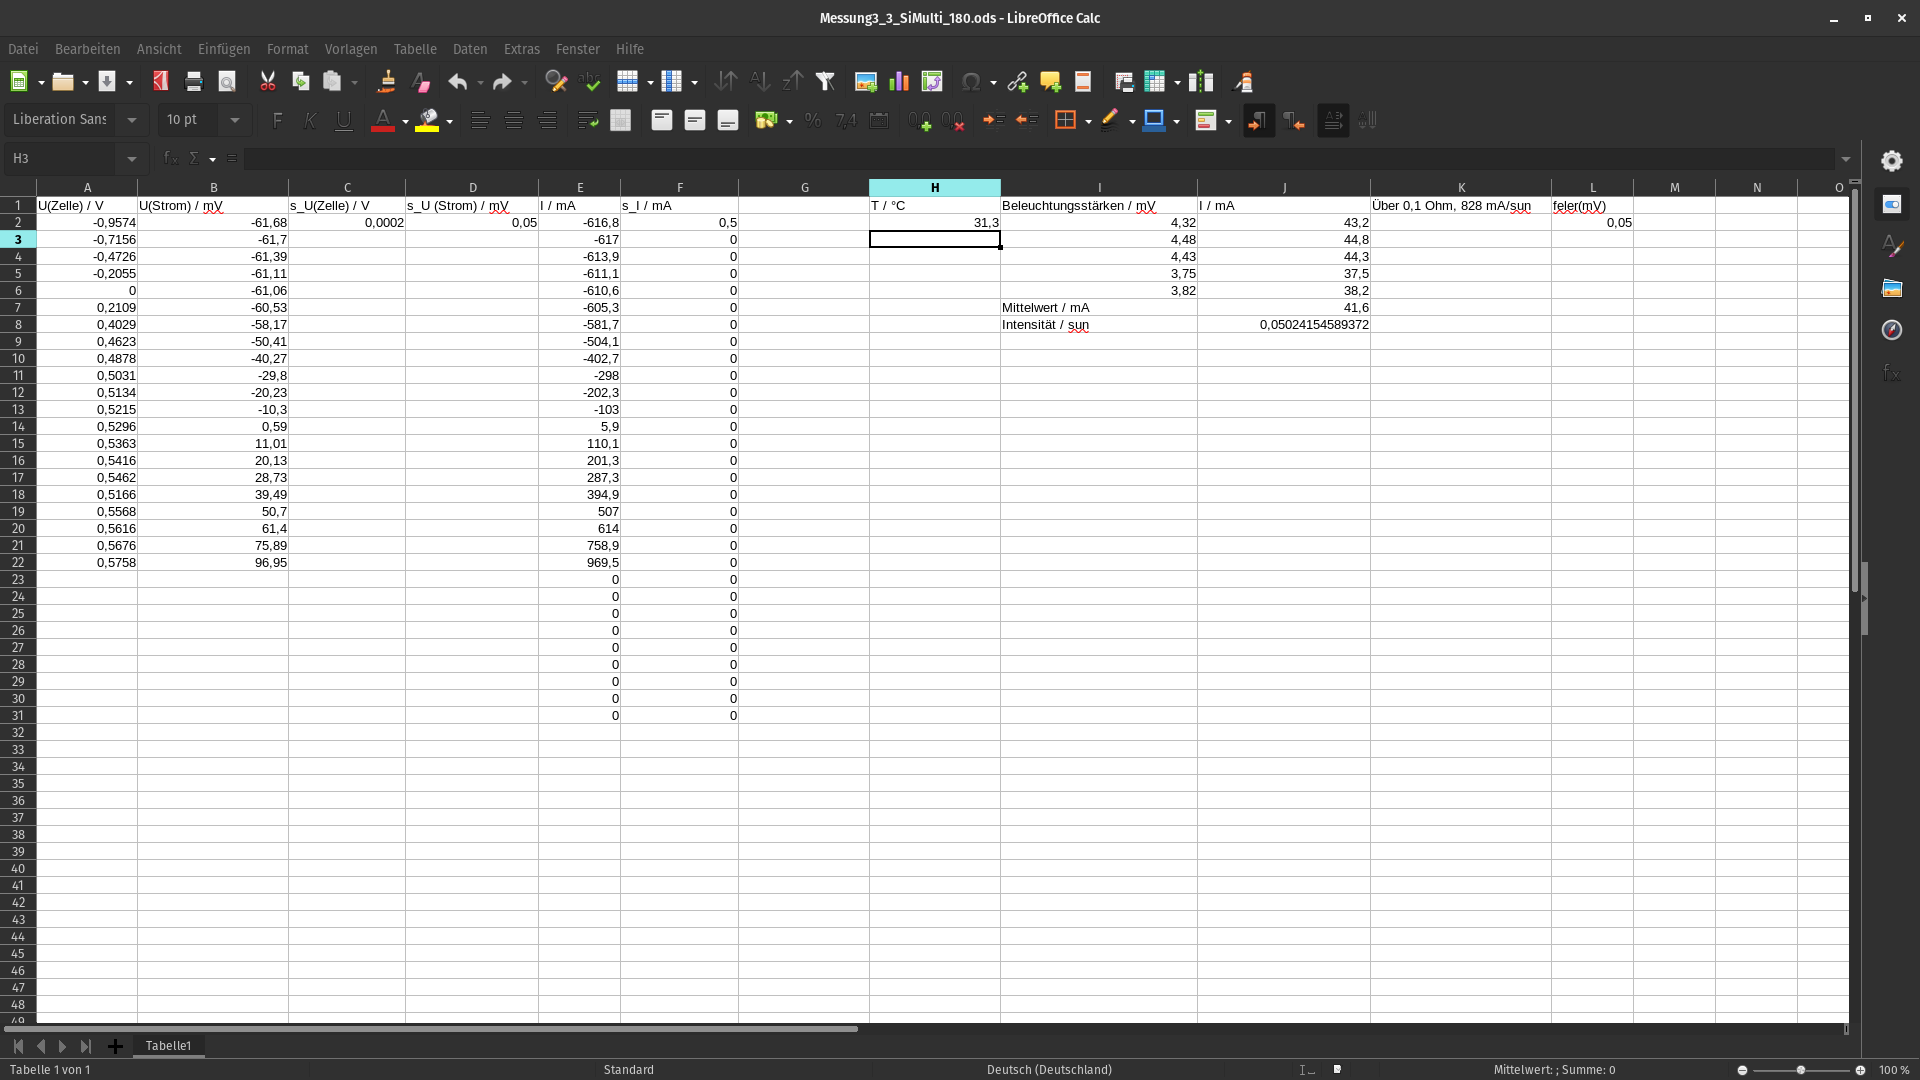
\includegraphics[angle = 90, width = 12cm]{Bilder/Daten/MessungMultiSi180.png}
    \caption{Beleuchtete Messung bei 180V am Stelltransformator an der Multi-Si-Zelle}
\end{figure}

\begin{figure}[h]
    \captionsetup{justification=centering,margin=2cm}
    \centering
    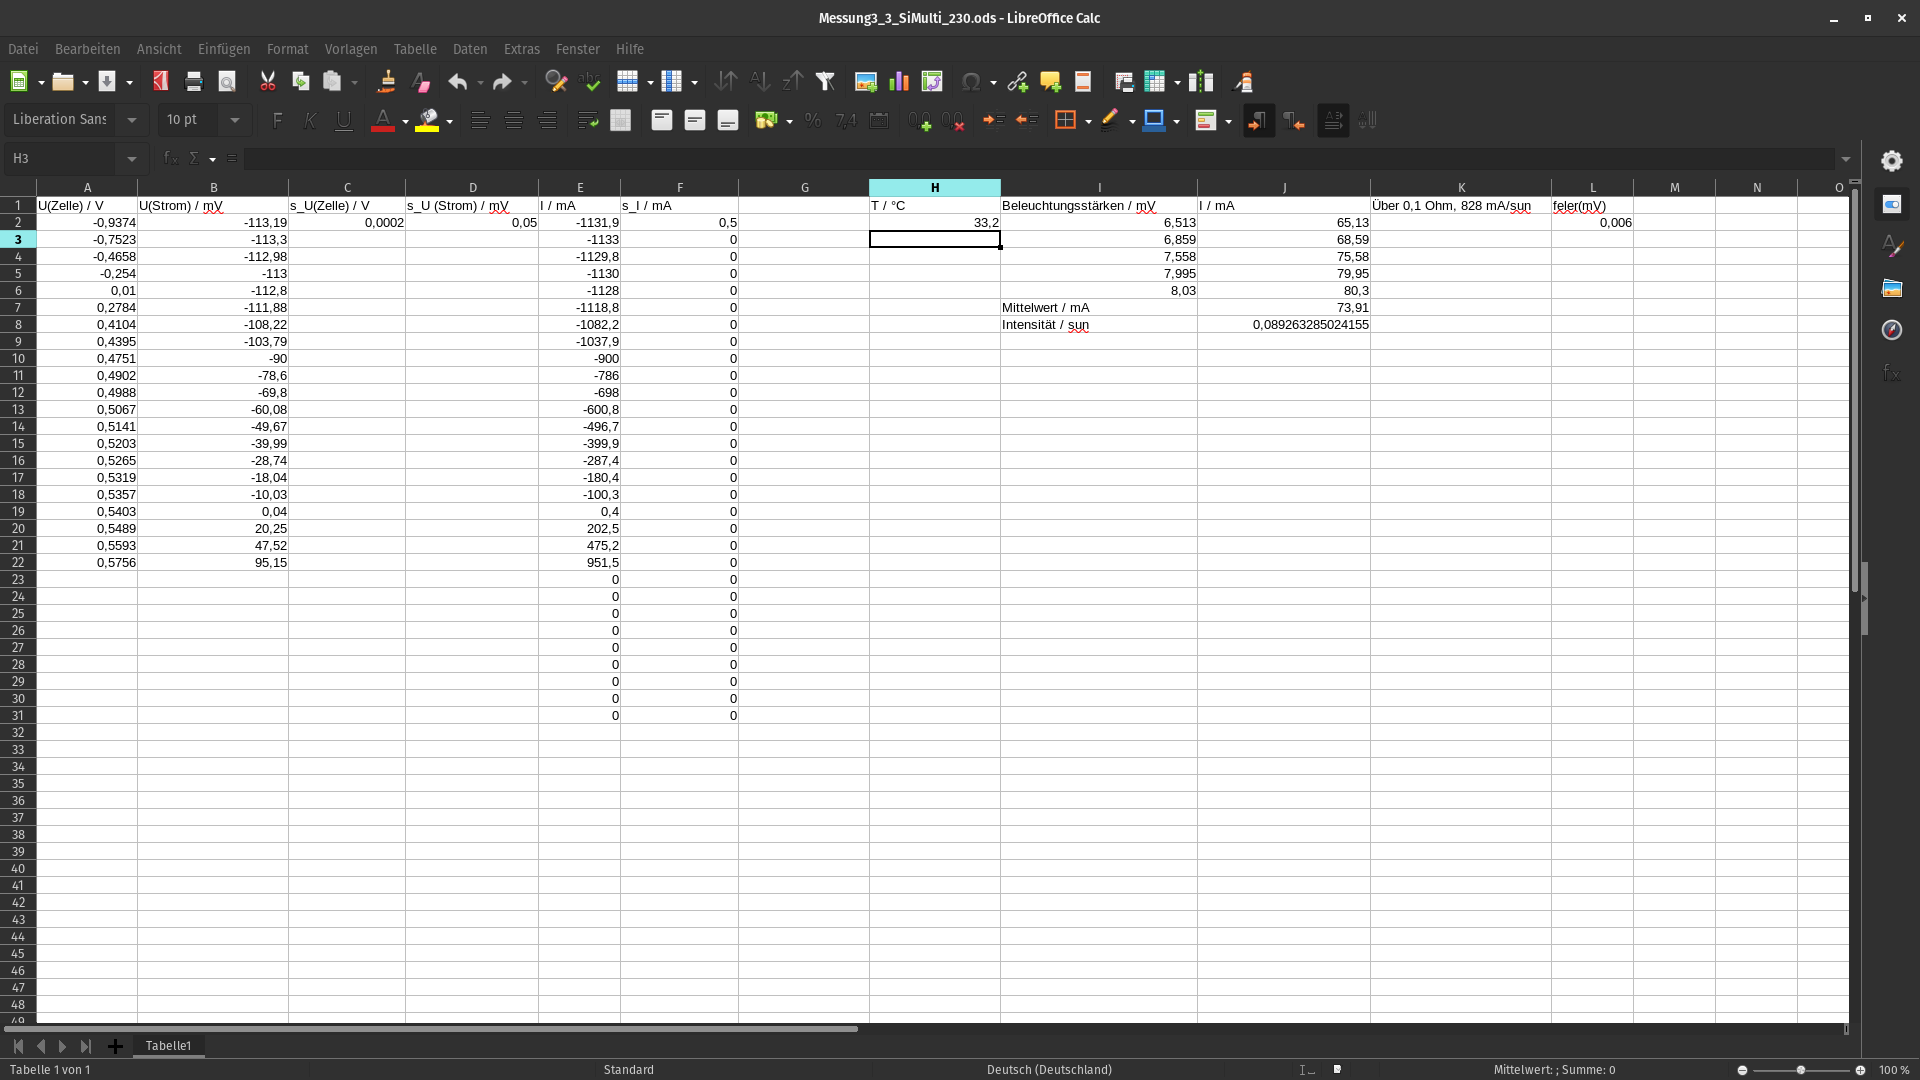
\includegraphics[angle = 90, width = 12cm]{Bilder/Daten/MessungMultiSi230.png}
    \caption{Beleuchtete Messung bei 230V am Stelltransformator an der Multi-Si-Zelle}
\end{figure}






\begin{figure}[h]
    \captionsetup{justification=centering,margin=2cm}
    \centering
    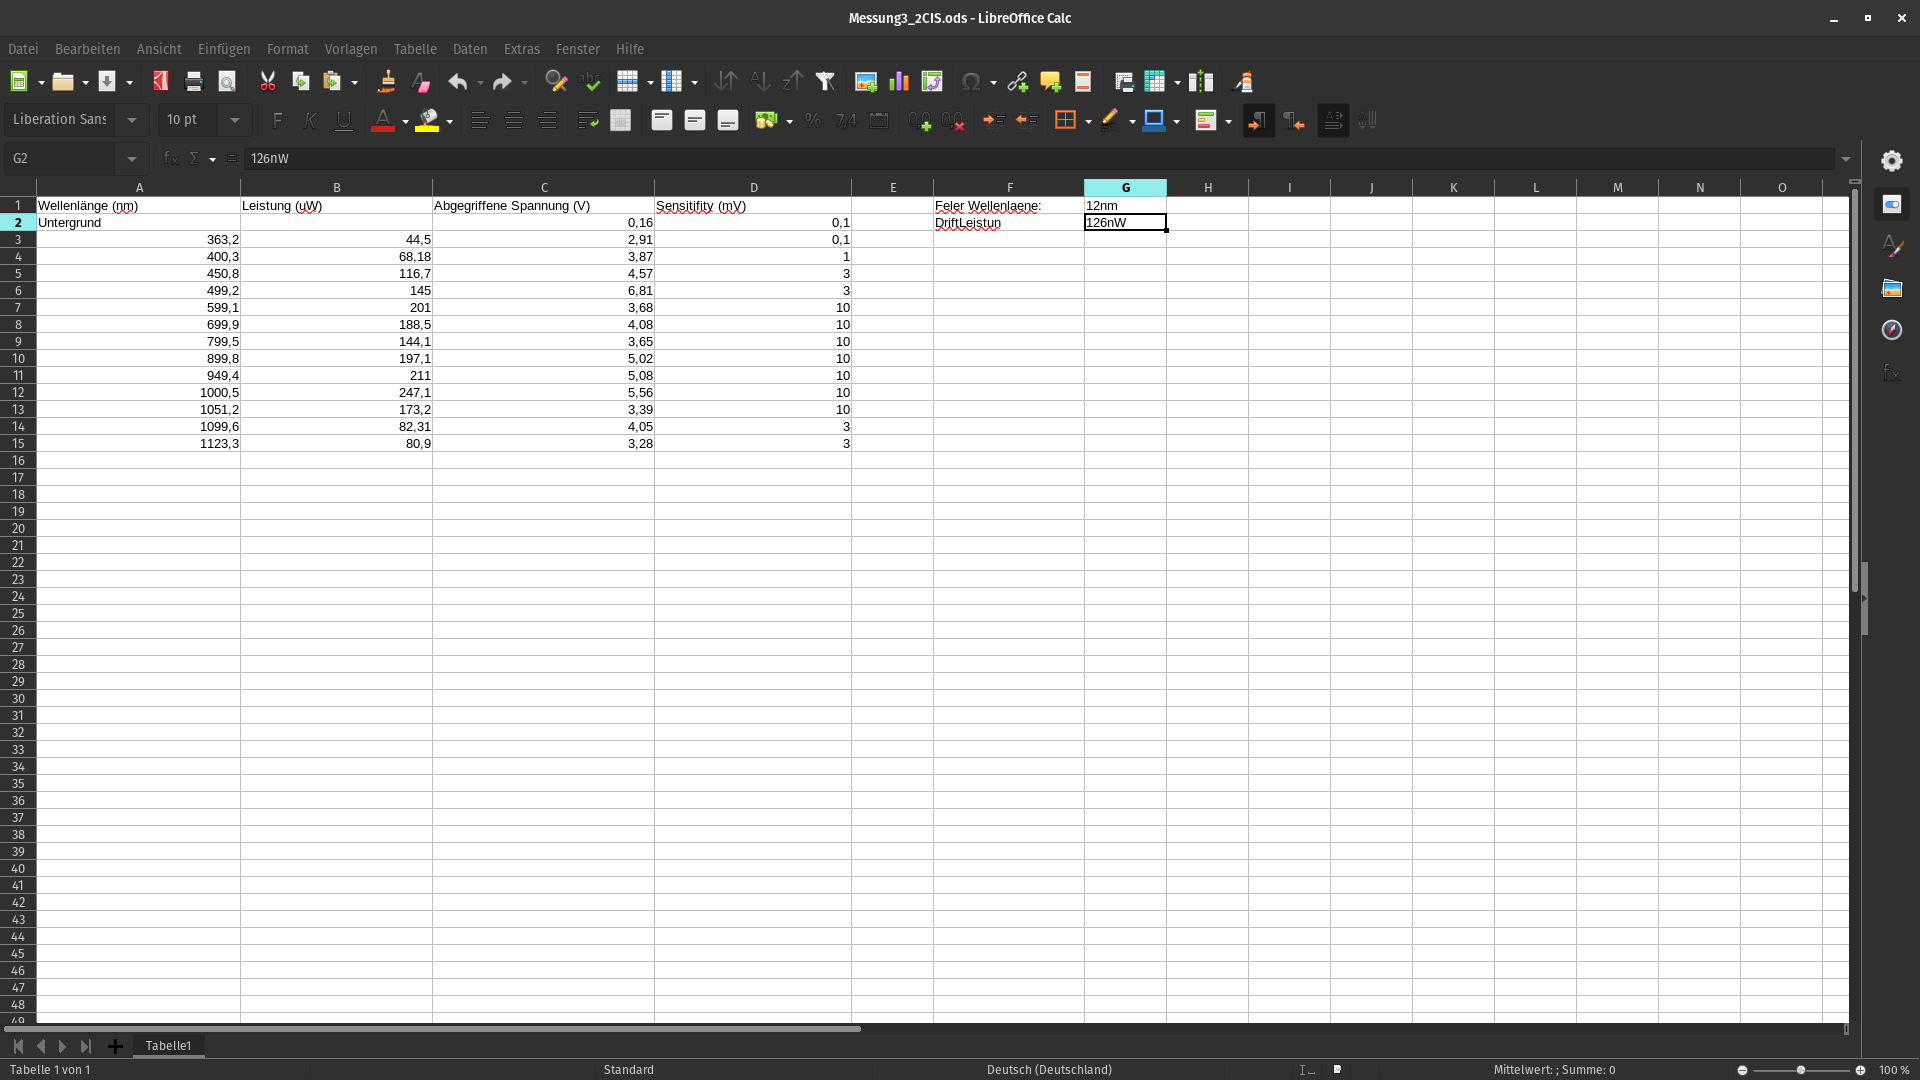
\includegraphics[angle = 90, width = 12cm]{Bilder/Daten/MessunngCIS.png}
    \caption{Messdaten zur Messung der spektralen Empfindlichkeit an der CIS-Zelle}
\end{figure}


\begin{figure}[h]
    \captionsetup{justification=centering,margin=2cm}
    \centering
    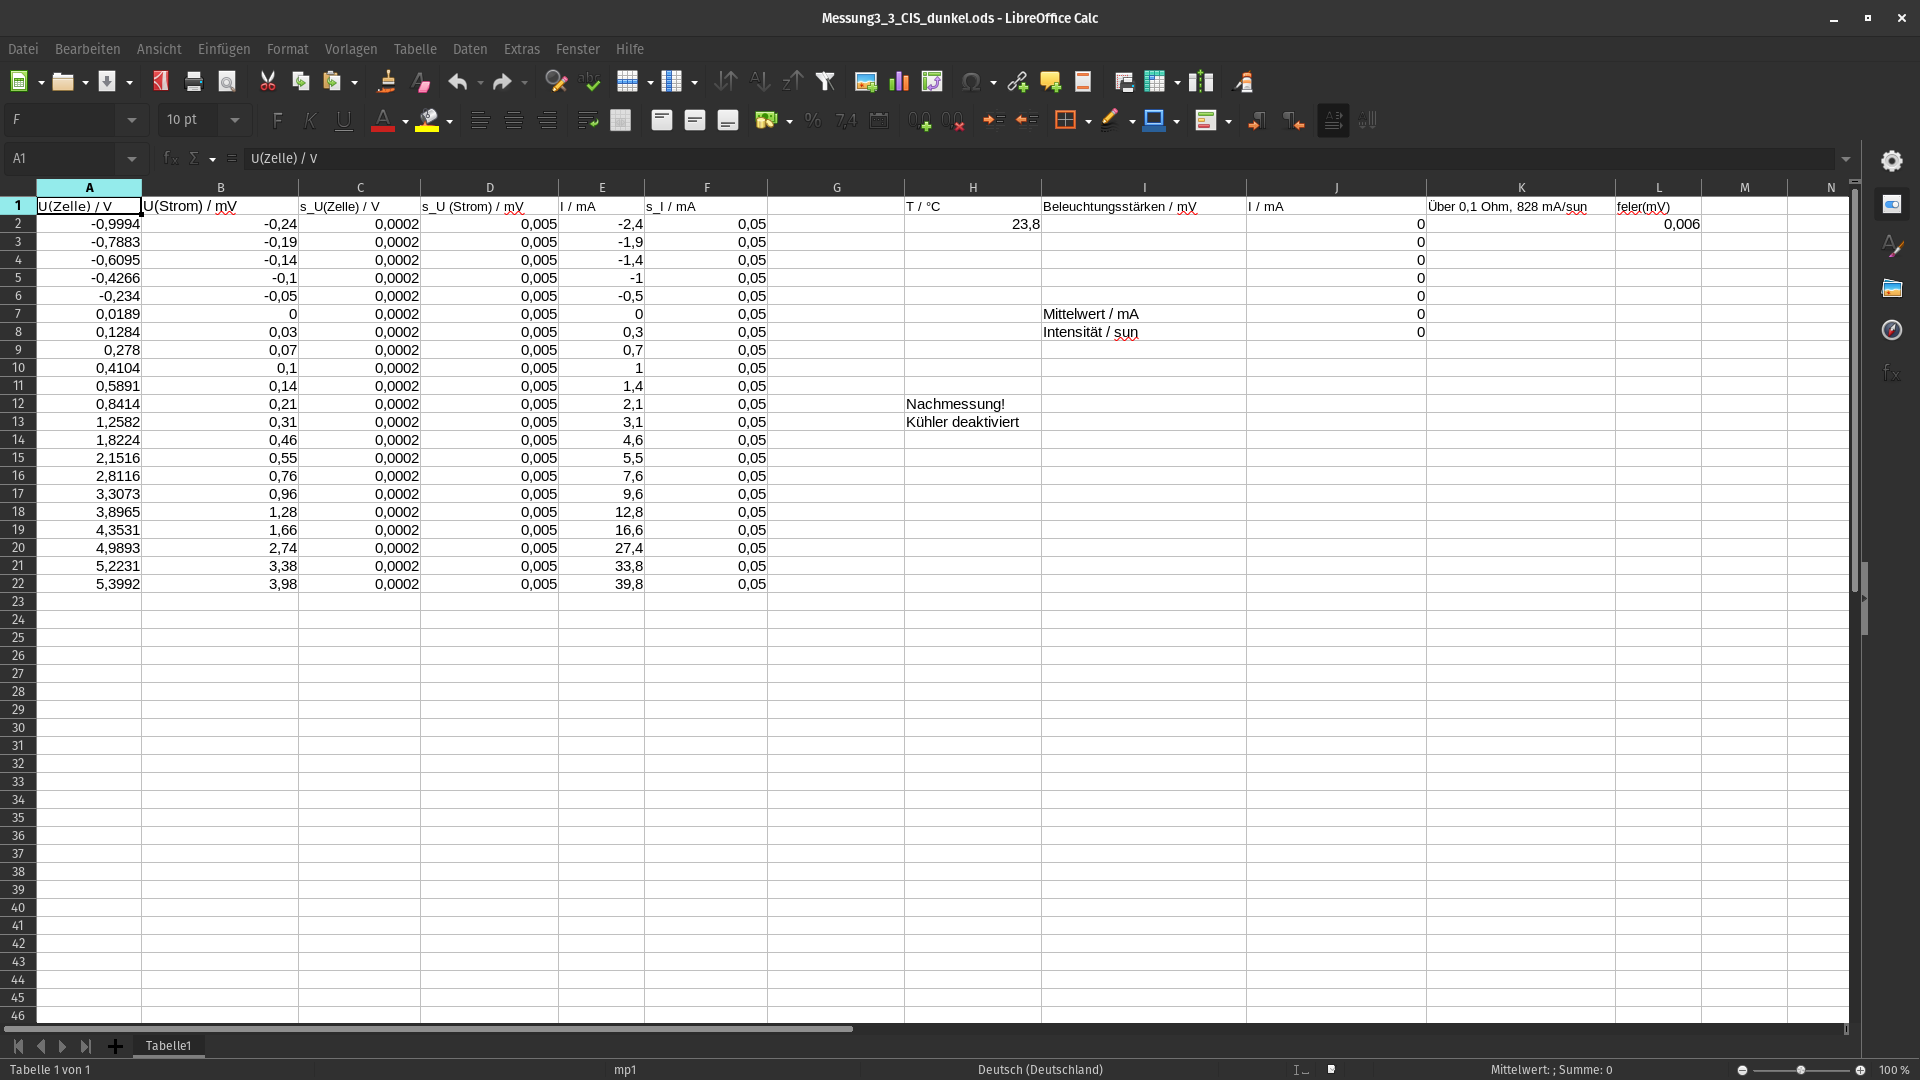
\includegraphics[angle = 90, width = 12cm]{Bilder/Daten/MessunngCISDunkel.png}
    \caption{Dunkelmessung an der CIS-Zelle}
\end{figure}

\begin{figure}[h]
    \captionsetup{justification=centering,margin=2cm}
    \centering
    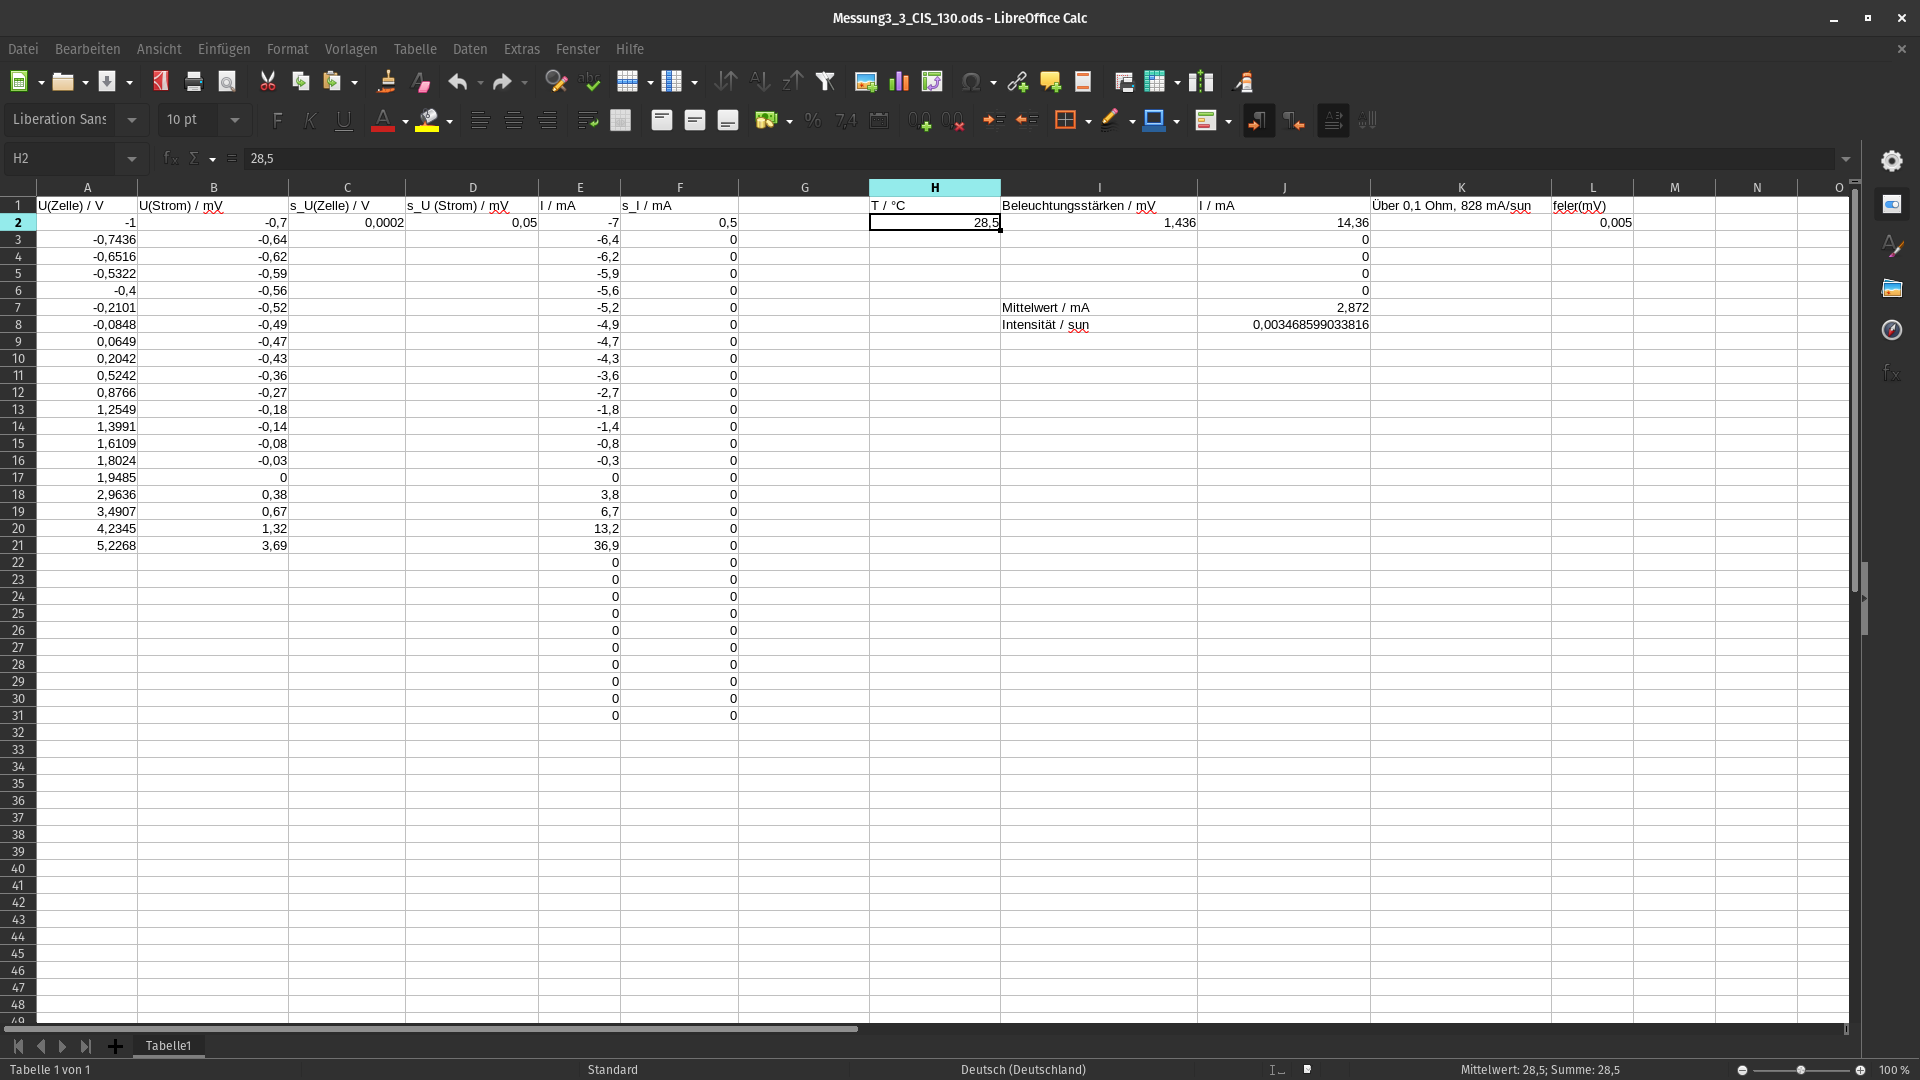
\includegraphics[angle = 90, width = 12cm]{Bilder/Daten/MessunngCIS130.png}
    \caption{Beleuchtete Messung bei 130V am Stelltransformator an der CIS-Zelle}
\end{figure}


\begin{figure}[h]
    \captionsetup{justification=centering,margin=2cm}
    \centering
    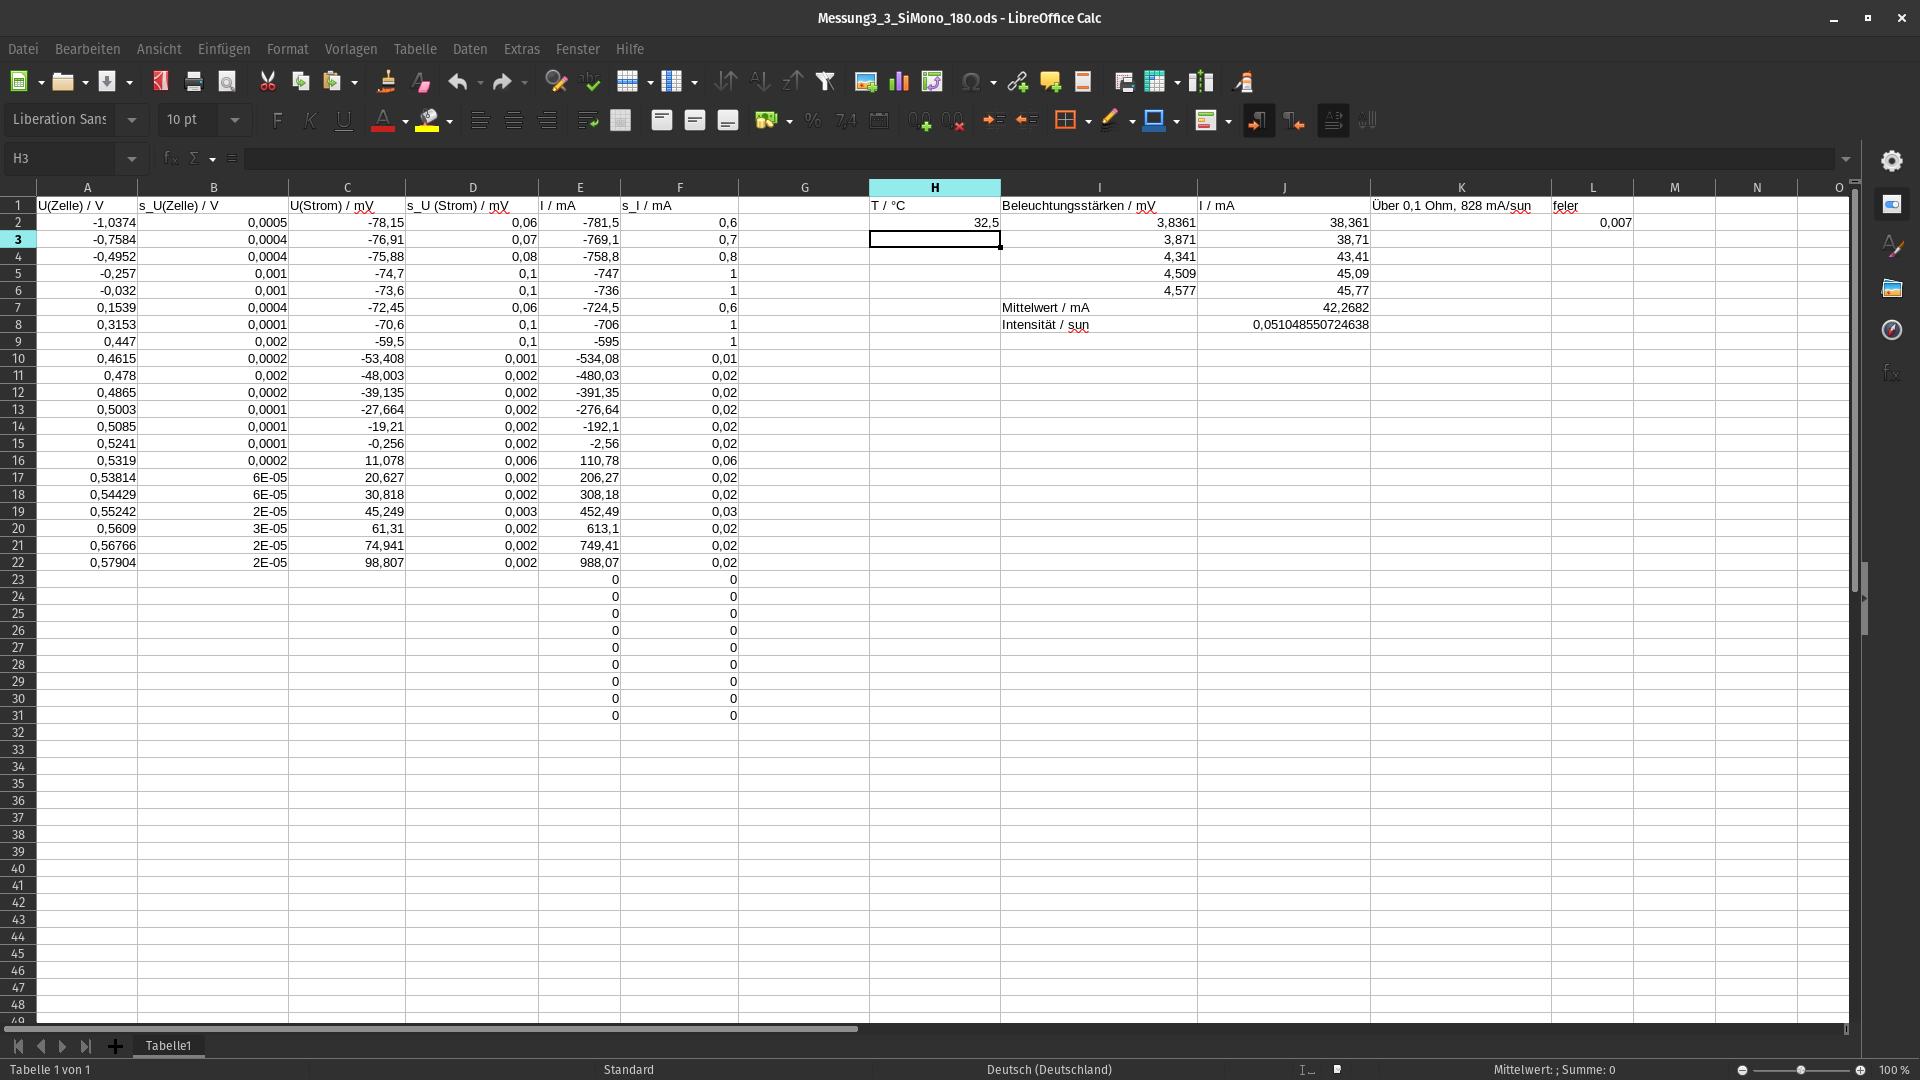
\includegraphics[angle = 90, width = 12cm]{Bilder/Daten/MessunngMonoSi180.png}
    \caption{Beleuchtete Messung bei 180V am Stelltransformator an der CIS-Zelle}
\end{figure}


\begin{figure}[h]
    \captionsetup{justification=centering,margin=2cm}
    \centering
    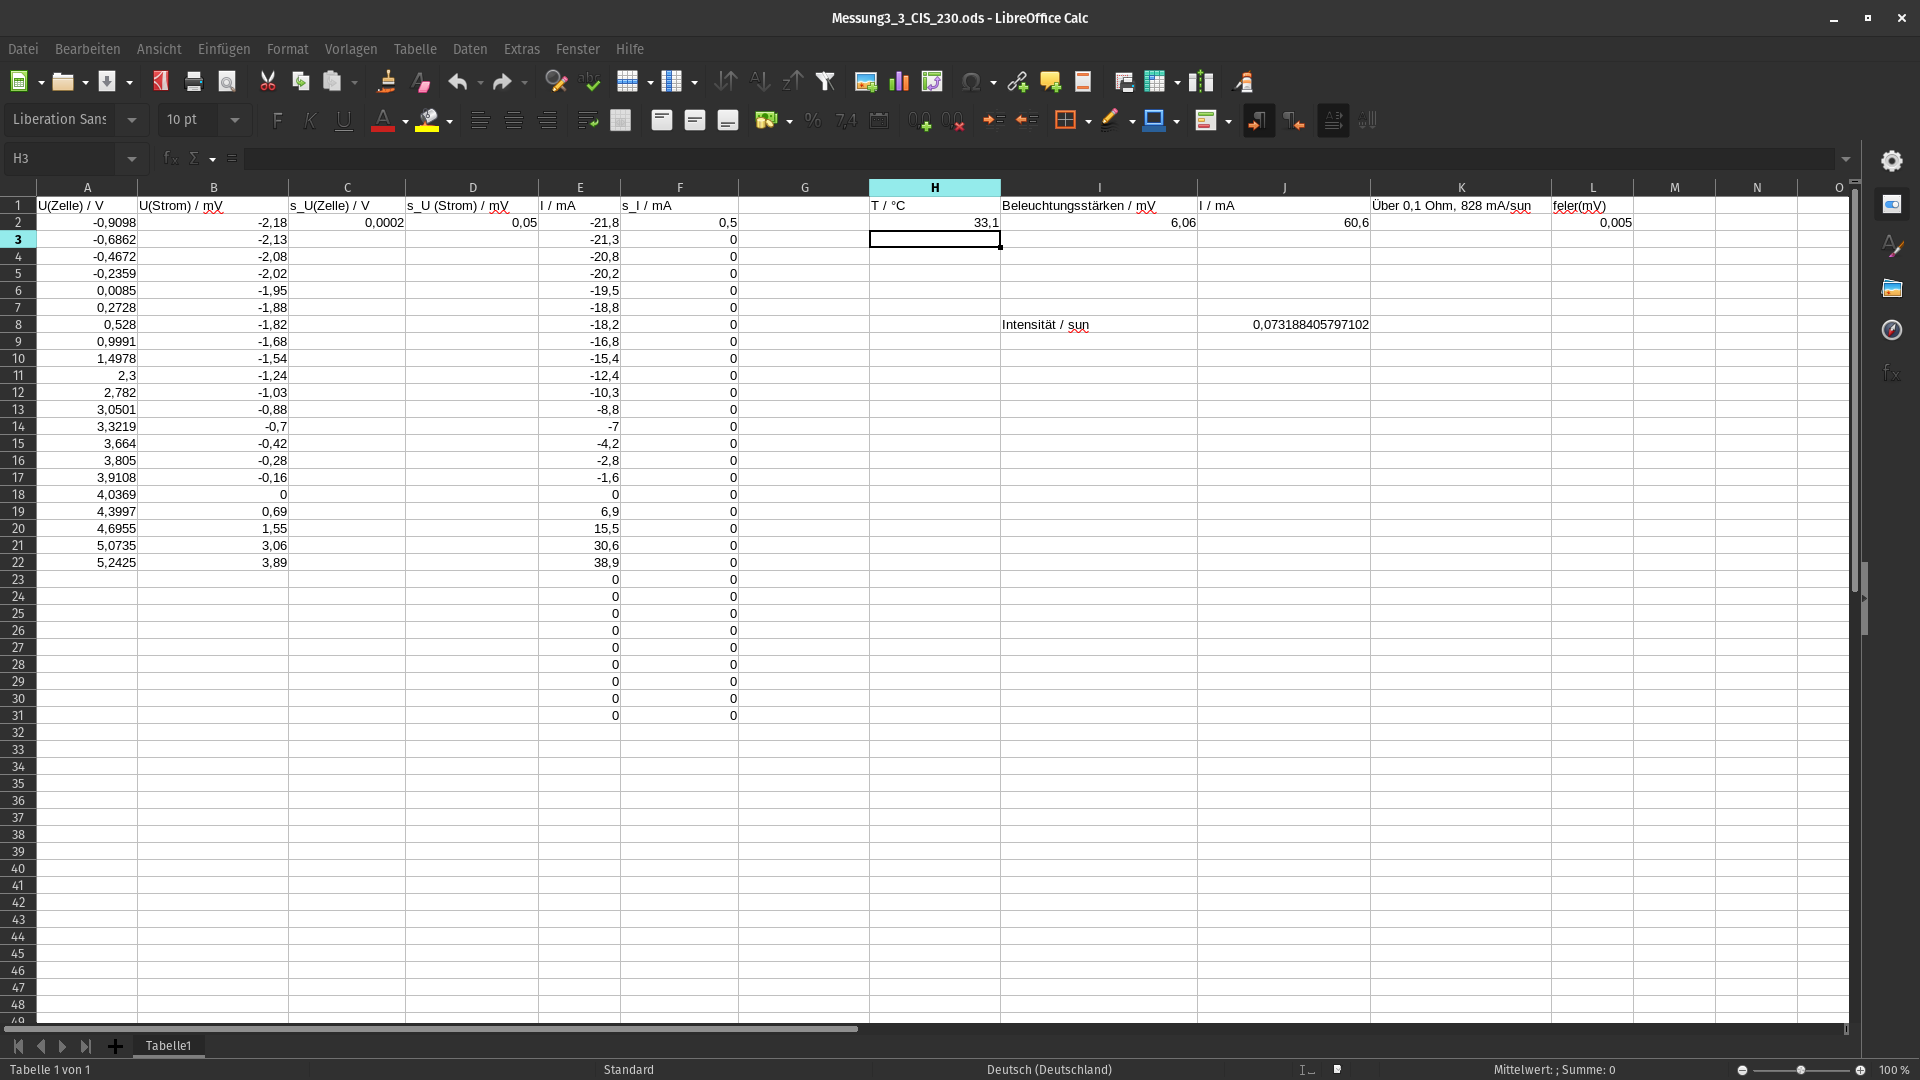
\includegraphics[angle = 90, width = 12cm]{Bilder/Daten/MessunngCIS230.png}
    \caption{Beleuchtete Messung bei 230V am Stelltransformator an der CIS-Zelle}
\end{figure}
